\documentclass[12pt,aspectratio=169]{beamer}
\usepackage[T2A,T1]{fontenc}
\usepackage[utf8]{inputenc}
\usepackage[english,russian]{babel}
\usepackage{amssymb,amsfonts,amsmath,mathtext}
\usepackage{cite,enumerate,float,indentfirst}
%\usepackage{hepunits}
\usepackage{siunitx}
\usepackage[customcolors,shade]{hf-tikz}
\usepackage{tikz}
\hypersetup{unicode=true}
\usepackage{xcolor}
\usepackage{beamerthemesplit}
\usepackage{tcolorbox}

% positioning textblocks
\usepackage[absolute, overlay]{textpos} 
\textblockorigin{0mm}{0mm} % start everything near the top-left corner

\definecolor{calmRed}{RGB}{191, 68, 72}
\definecolor{calmGreen}{RGB}{107, 172, 102}
\definecolor{calmBlue}{RGB}{62, 124, 178}
\definecolor{calmYellow}{RGB}{223, 215, 100}
\definecolor{calmOrange}{RGB}{249, 146, 70}
\definecolor{gray}{RGB}{127,127,127}
\definecolor{calmGray}{RGB}{100,100,100}

\newcommand*{\advisors}[1]{\def\@advisors{#1}}

\setbeamerfont{itemize/enumerate body}{}
\setbeamerfont{itemize/enumerate subbody}{size=\small}
\setbeamerfont{itemize/enumerate subsubbody}{size=\small}

\usetikzlibrary{arrows,backgrounds,decorations.pathmorphing}

\usepackage{graphicx}

\graphicspath{{images/}}




\usetheme{Madrid}
\usefonttheme[onlymath]{serif}
\usecolortheme[named=calmBlue]{structure}
\setbeamercolor{footline}{fg=calmBlue}
\setbeamercolor{section in head/foot}{fg=white, bg=black}


\newcommand{\backupbegin}{
	\newcounter{finalframe}
	\setcounter{finalframe}{\value{framenumber}}
}
\newcommand{\backupend}{
	\setcounter{framenumber}{\value{finalframe}}
}

\setbeamertemplate{itemize items}[circle]
\setbeamertemplate{enumerate items}[circle]


\setbeamertemplate{footline}{
  \leavevmode%
  \hbox{%
  \begin{beamercolorbox}[wd=.333333\paperwidth,ht=2.25ex,dp=1ex,center]{}%
   Степан Захаров, ФФ НГУ
  \end{beamercolorbox}%
  \begin{beamercolorbox}[wd=.333333\paperwidth,ht=2.25ex,dp=1ex,center]{}%
    Новосибирск, 2021
  \end{beamercolorbox}%
  \begin{beamercolorbox}[wd=.333333\paperwidth,ht=2.25ex,dp=1ex,right]{}%
  Слайд \insertframenumber{} из \inserttotalframenumber \hspace*{2ex}
  \end{beamercolorbox}}%
  \vskip0pt%
}

%%% Title page %%%
\setbeamertemplate{title page}{
	\vbox{}
	\vfill
	\begin{centering}
		{\usebeamercolor[fg]{titlegraphic}\inserttitlegraphic\par}\vskip1em
		{\rmfamily\textsc{--- Магистерская диссертация --- }\par}\vskip1em
		\begin{beamercolorbox}[sep=8pt,center,rounded=true,shadow=true]{title}
			\usebeamerfont{title}\inserttitle\par%
		\end{beamercolorbox}%
		\vskip1em\par
		\begin{beamercolorbox}[sep=7pt,center]{author}
			\usebeamerfont{author}
			\textbf{Докладчик:}\par
			\insertauthor
			\ifx\@advisors\@empty\else                                  
			\par\medskip\textbf{Научный руководитель:}\par\def\and{\par}\@advisors 
			\fi                                                        
		\end{beamercolorbox}
		\begin{beamercolorbox}[sep=7pt,center]{date}
			\usebeamerfont{date}\insertdate
		\end{beamercolorbox}
	\end{centering}
	\vfill
}
\makeatother

\newcommand{\itemi}{\item[\checkmark]}
\title{\Large{Лазерный поляриметр --- система измерения поляризации электронного пучка коллайдера ВЭПП--4М}}
\author{Степан Алексеевич Захаров}
\advisors{к.ф.-м.н.,~с.н.с.~ИЯФ~СО~РАН Иван~Борисович~Николаев}
\date{\today}

\tikzstyle{every picture}+=[remember picture]
\tikzstyle{na} = [baseline=-.5ex]

\begin{document}

\maketitle

%\begin{frame}[t]
%	\frametitle{План работ}
%	\begin{itemize}
%		\item[\color{calmGreen}$\checkmark$] \textit{Сентябрь -- Декабрь 2019:} сборка системы и написание программного пакета для работы с ней
%		\item[\color{calmGreen}$\checkmark$]\textit{Сентябрь -- Ноябрь 2020:} отработка процесса измерения поляризации пучков
%		\item[\color{calmRed}$\Rightarrow$] \textit{Ноябрь 2020 -- Январь 2021:} калибровки энергии с использованием новой ССОД в области $\Upsilon-\text{резонанса}$\\ \color{calmRed}{Перенесены на февраль в связи с остановкой комплекса =(} \color{black}
%		\item[\color{calmOrange}$\Rightarrow$] \textit{Ноябрь 2020 -- Январь 2021:} Изучение систематик метода и путей борьбы с ними
%		\item[\color{calmGreen}$\Rightarrow$] \textit{Ноябрь 2020 -- Апрель 2021:} подготовка дипломной работы
%	\end{itemize}
%\end{frame}

%\begin{frame}[t]
%	\frametitle{План доклада}
%			\begin{itemize}
%				\onslide<1-> \item \textcolor<2-7>{calmGray}{Обоснование необходимости в прецизионных измерениях $E$}
%				\onslide<2-> \item \textcolor<3-7>{calmGray}{Обзор существующих методов: мотивация использования метода измерения $E$ по асимметрии обратного комптоновского рассеяния}
%				\onslide<3-> \item \textcolor<4-7>{calmGray}{Теория обратного комптоновского рассеяния}
%				\onslide<4-> \item \textcolor<5-7>{calmGray}{Принцип работы лазерного поляриметра}
%				\onslide<5-> \item \textcolor<6-7>{calmGray}{Измерение и контроль поляризации оптических пучков}
%				\onslide<6-> \item \textcolor<7>{calmGray}{Сбор и обработка данных, определение эффекта поляризации электронного пучка}
%				\onslide<7-> \item Анализ ошибок метода
%				\onslide<8>\item {Обзор полученных результатов}
%				
%				
%						
%		\end{itemize}
%\end{frame}


\begin{frame}
	\frametitle{Комплекс ВЭПП-4М --- КЕДР}
	\begin{minipage}[c]{0.49\linewidth}
		\begin{center}
			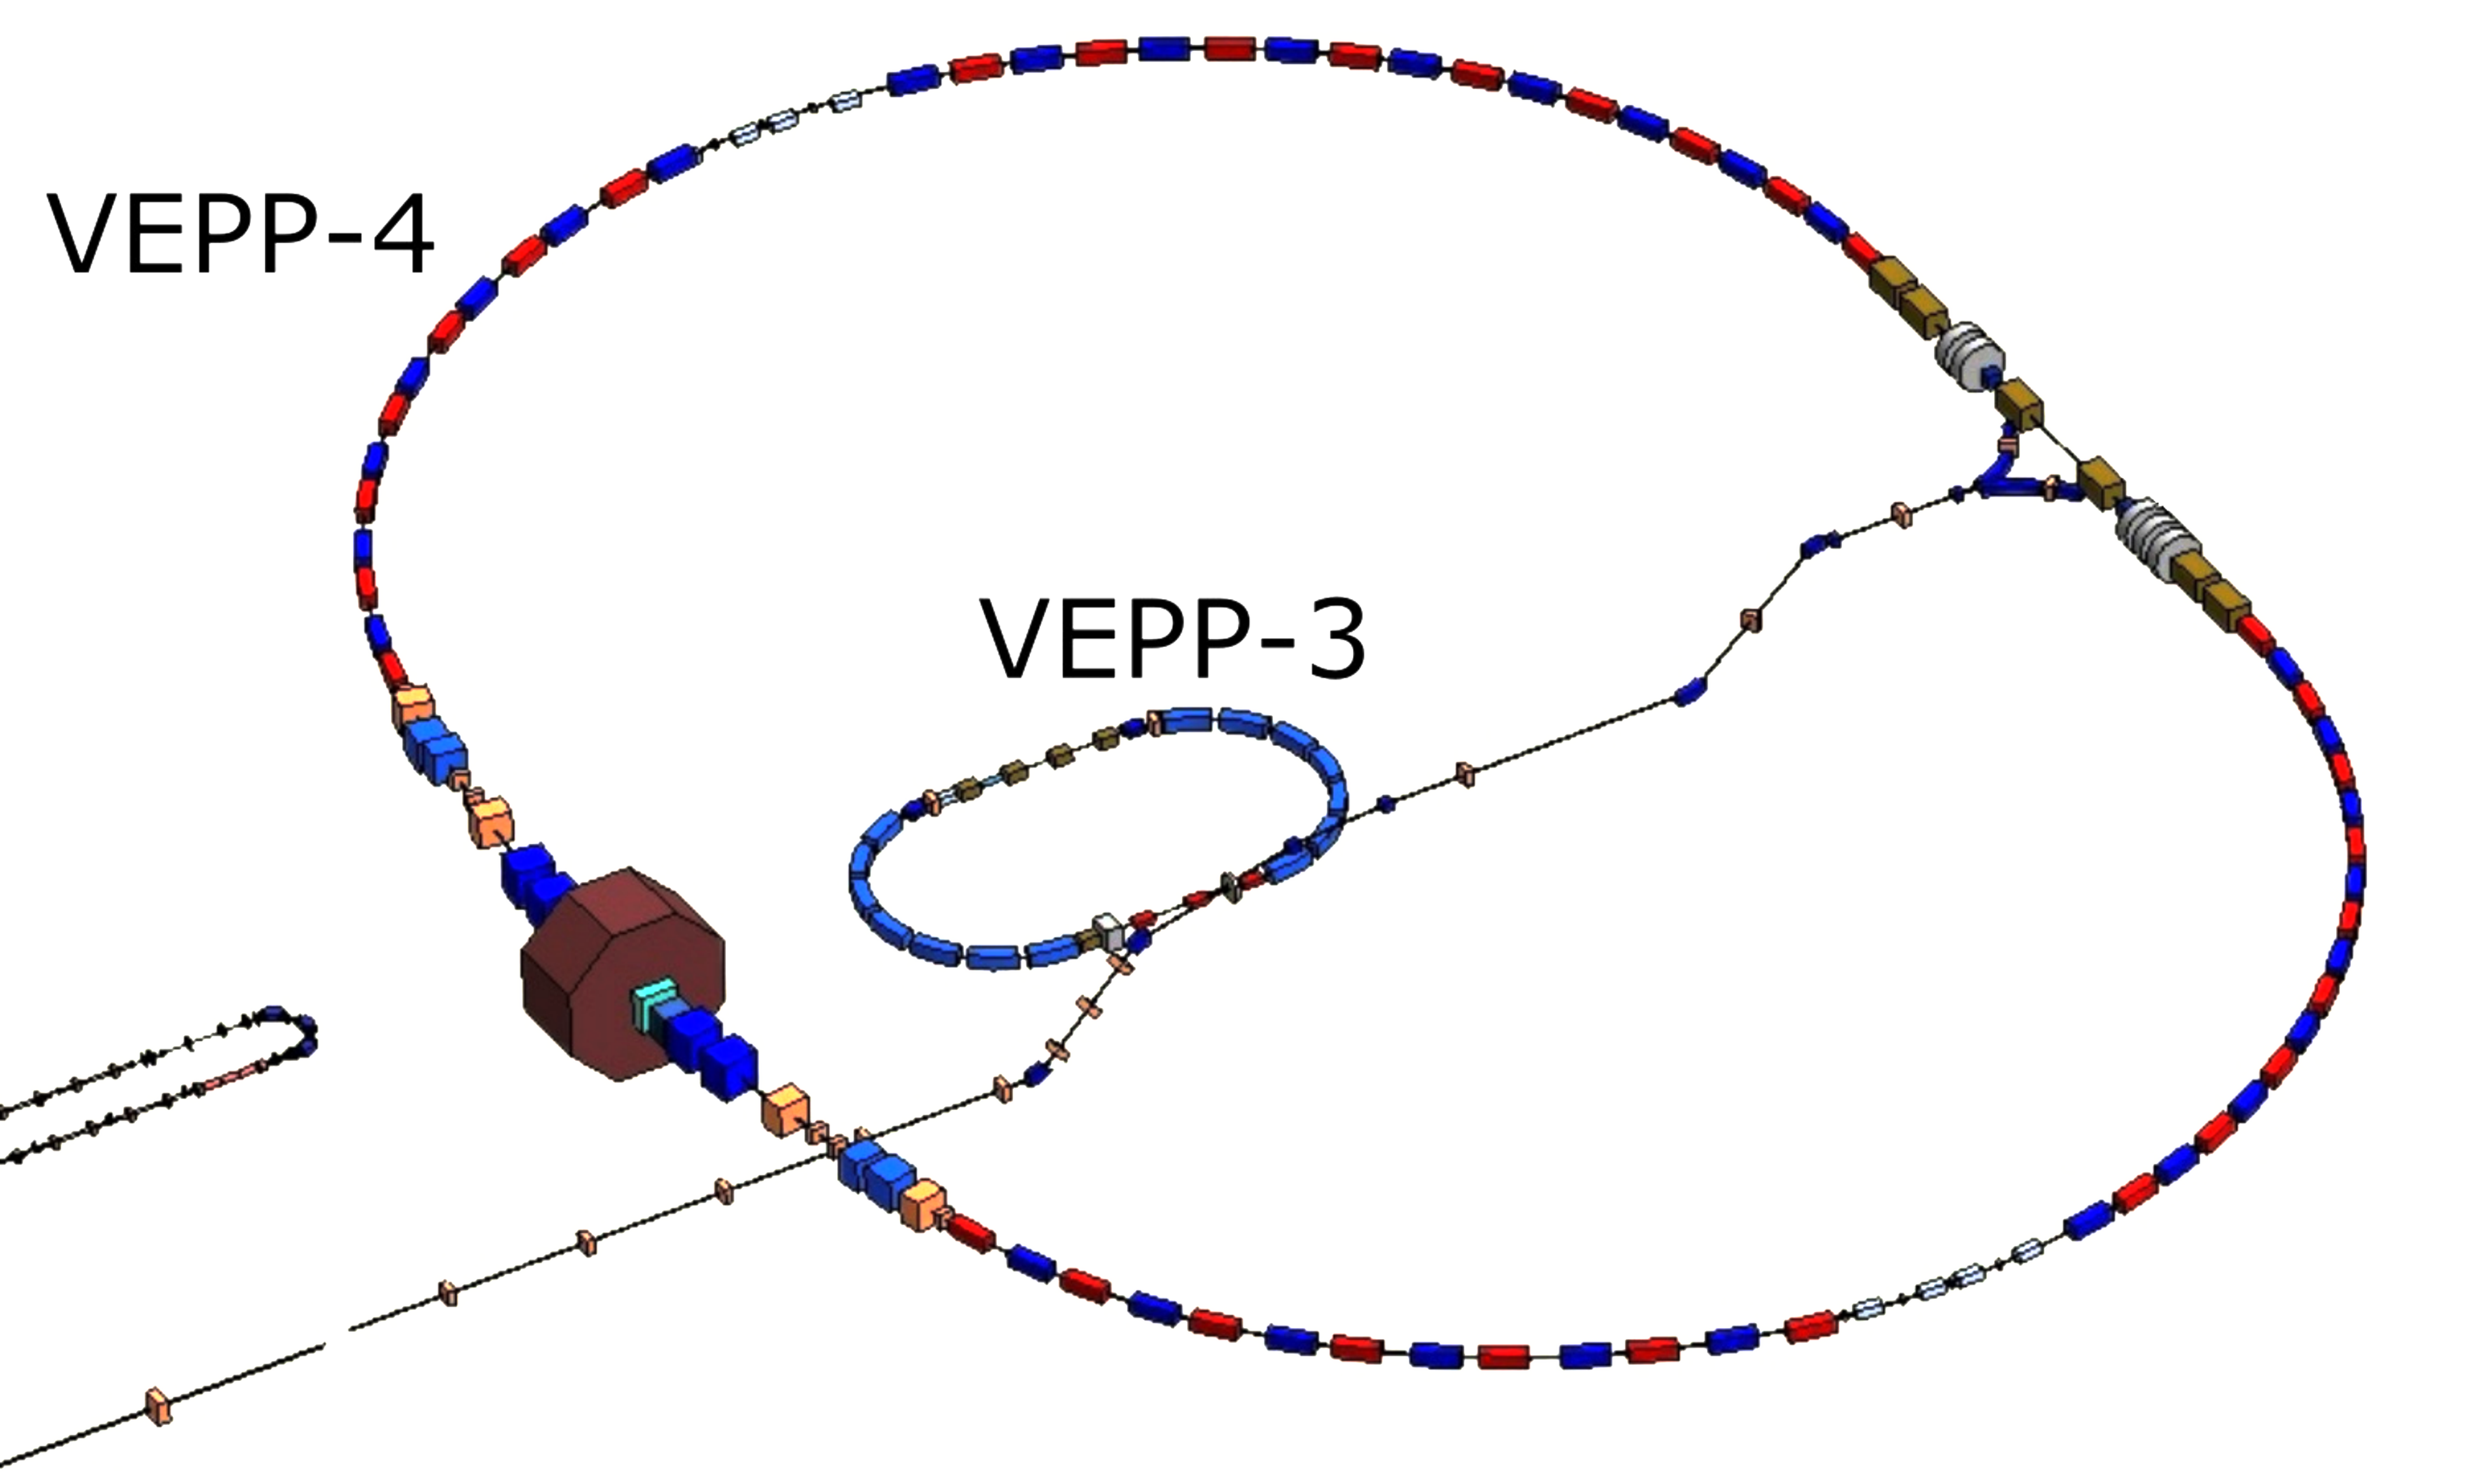
\includegraphics[width=1\linewidth]{VEPP-4.pdf}
			\footnotesize{Коллайдер ВЭПП-4М}
		\end{center}
	\end{minipage}
	\begin{minipage}[h]{0.49\linewidth}
		\begin{center}
			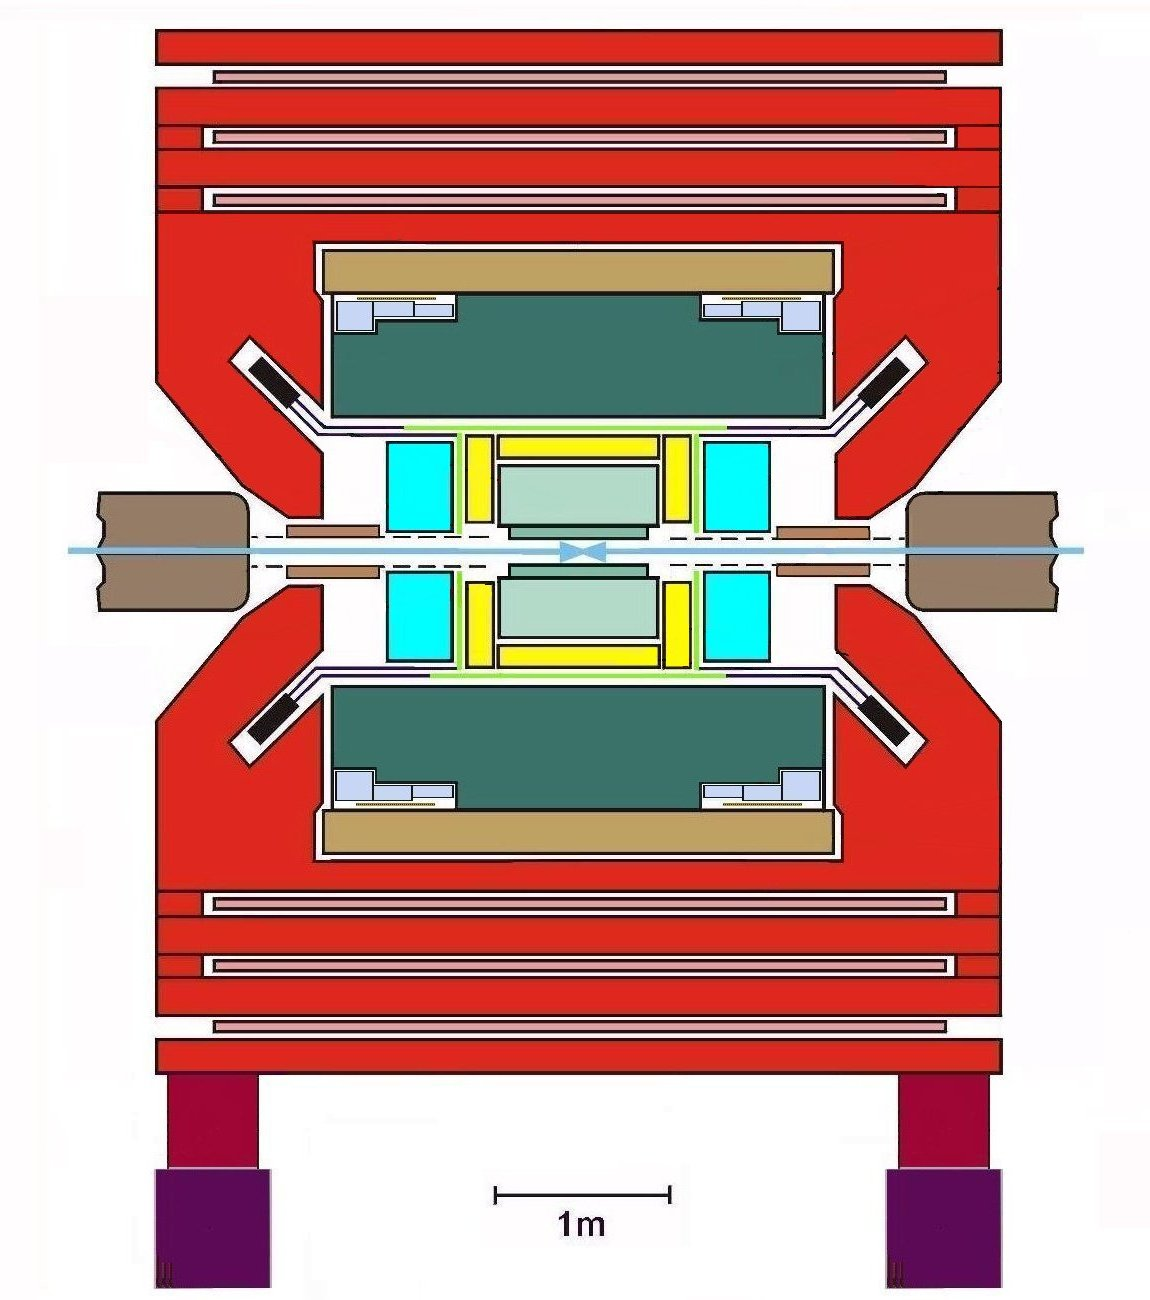
\includegraphics[width=0.6\linewidth]{KEDR.jpg}\\
			\footnotesize{Детектор КЕДР}
		\end{center}
		
	\end{minipage}
\end{frame}

\begin{frame}
	\frametitle{Мотивация}
	\begin{minipage}[h]{0.55\linewidth}
			\begin{itemize}
				\itemsep=0.7em
				\item Экспериментальная программа детектора КЕДР $\rightarrow$ измерения масс в области $\Upsilon-\text{резонанса}$
				\onslide<2-> \item Необходимость в прецизионном измерении энергии пучков
				\onslide<3-> \item [\textcolor{calmGreen}{\checkmark}] В ИЯФ накоплен большой опыт по различным методам измерения энергии
				\onslide<4>\item [$\Rightarrow$] Создание новой установки <<Лазерный поляриметр>>
		\end{itemize}
		\hfill
	\end{minipage}
	\begin{minipage}[h]{0.43\linewidth}
		\onslide<1->\ 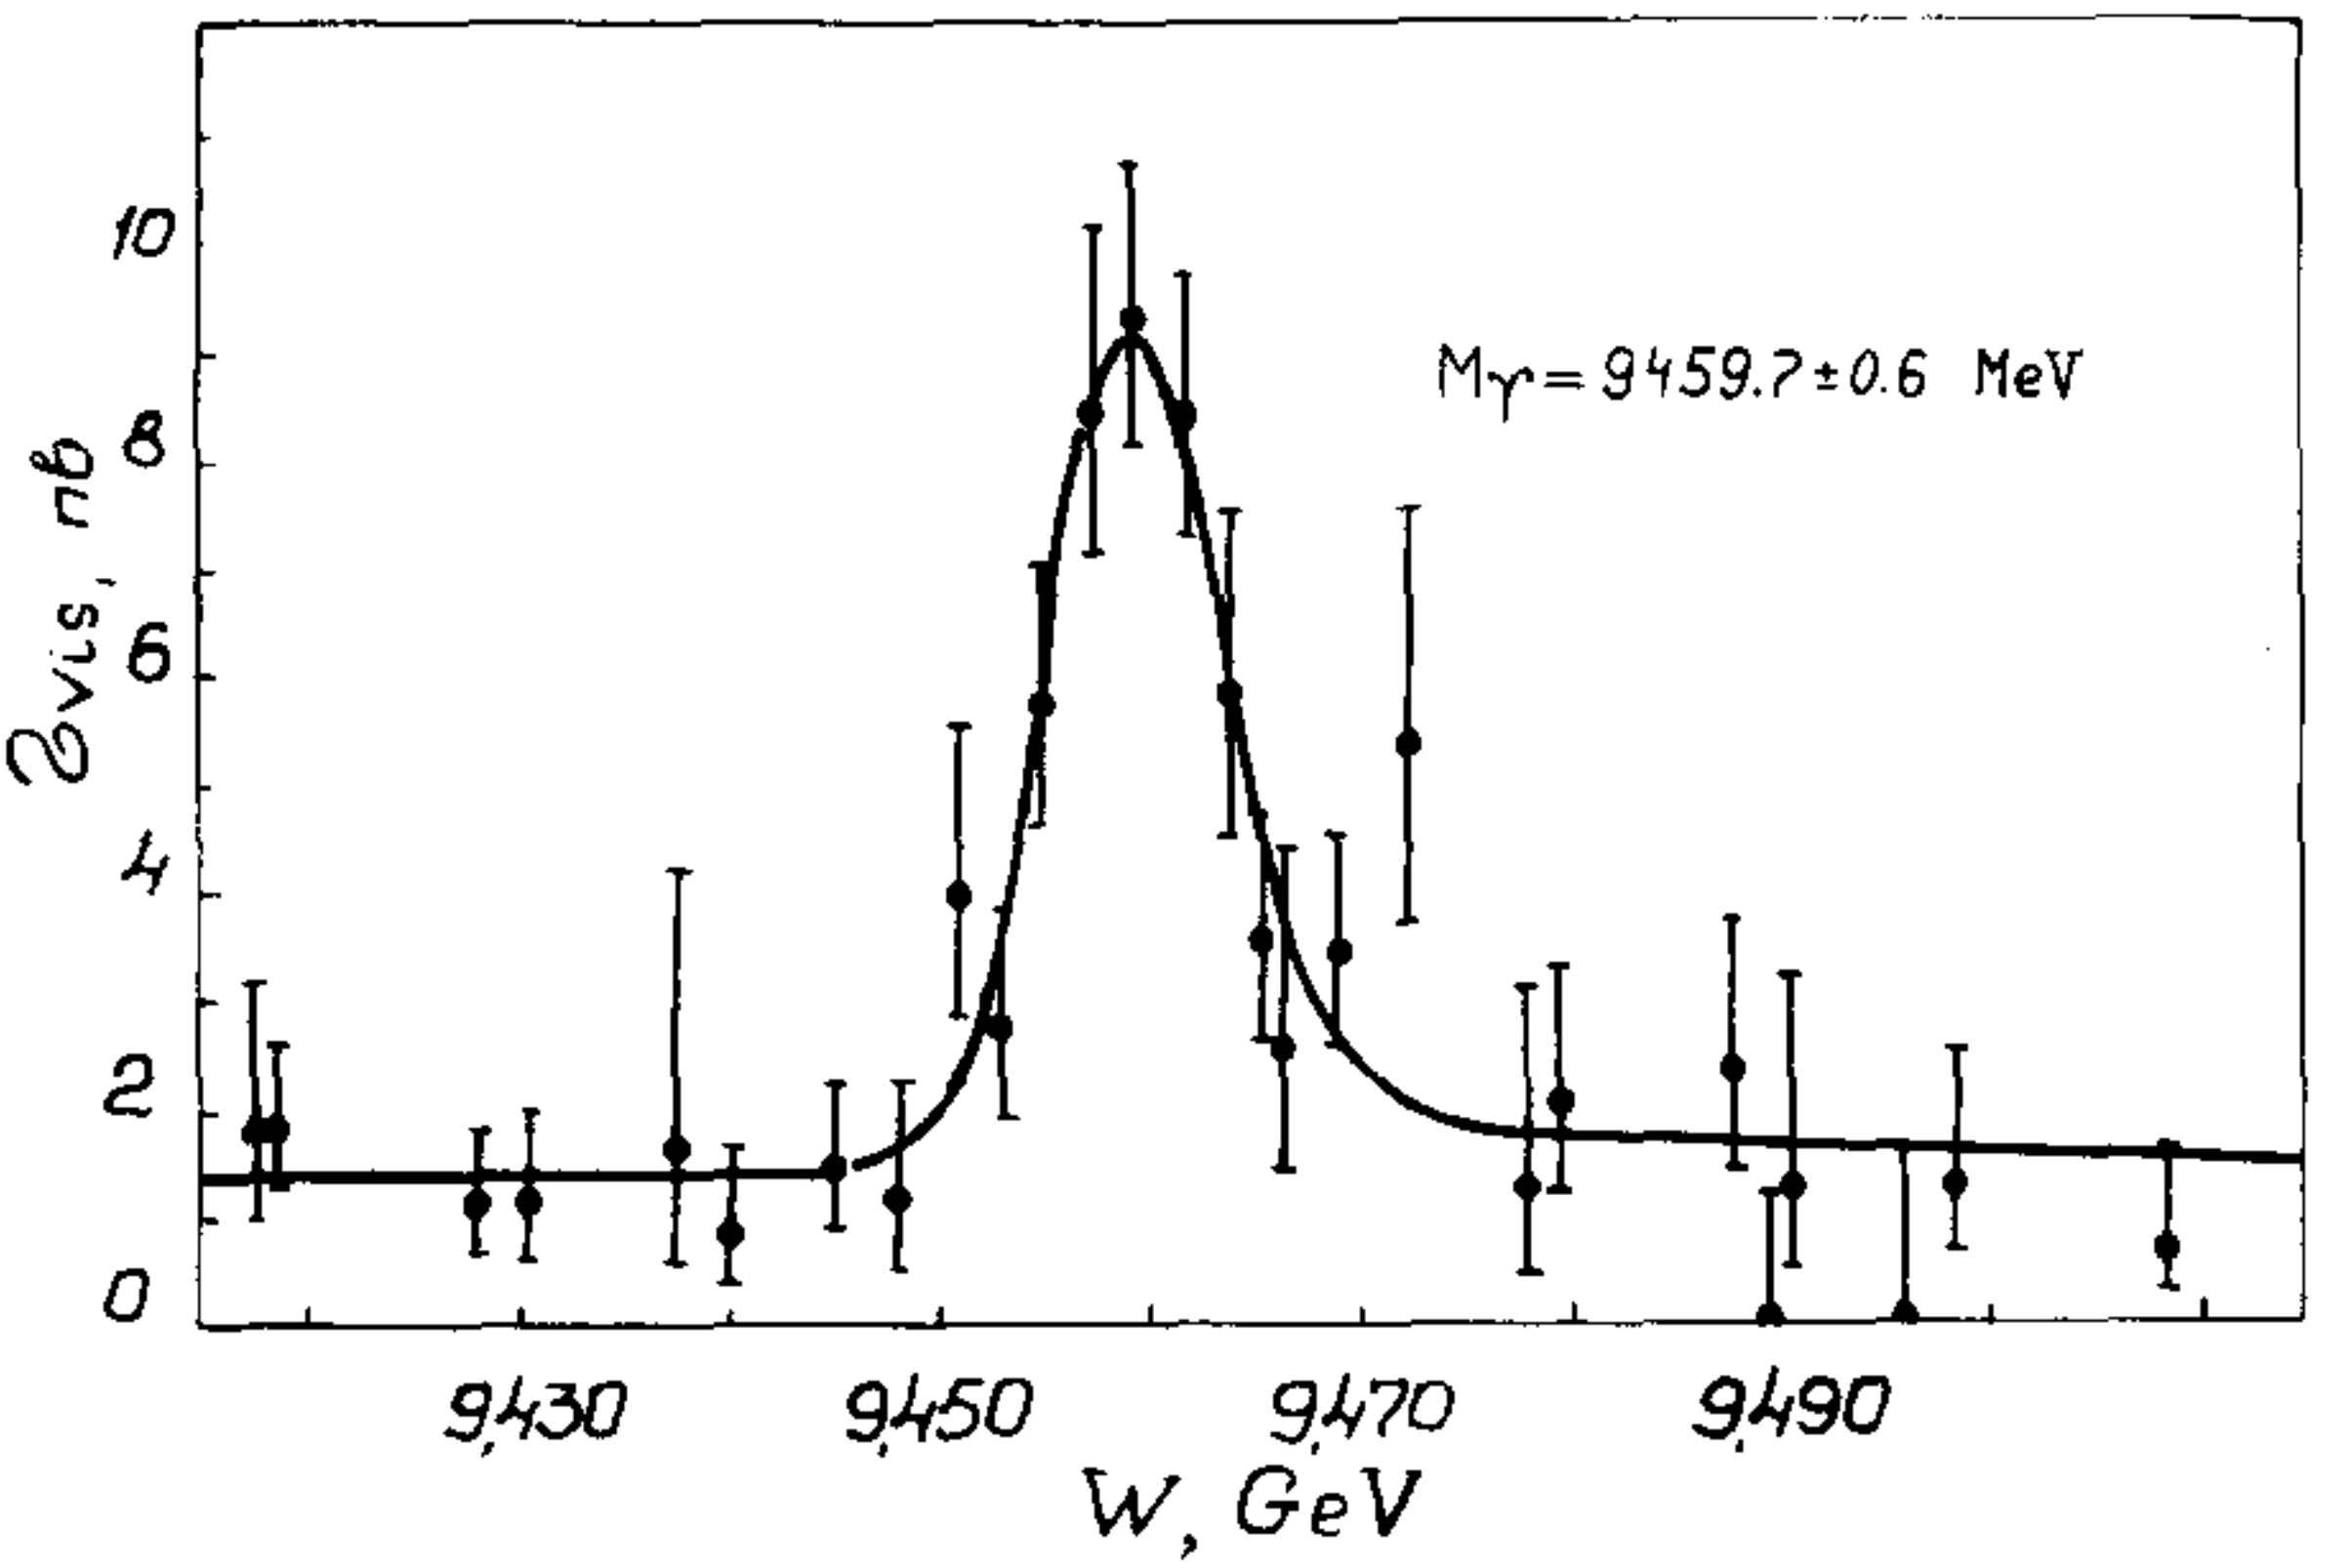
\includegraphics[width=1\linewidth]{UpsilonMass.png}
		\\\tiny{Рисунок из статьи: A.S. Artamonov \emph{et al.}, High Precision Measurement of the Y Meson Mass, 1982}
	\end{minipage}
\end{frame}






\begin{frame}[t]
	\frametitle{Рассеяние поляризованных фотонов на поляризованных электронах}
		\begin{tikzpicture}[
		>=stealth',
		pos=.8,
		photon/.style={decorate,decoration={snake,post length=1mm}},
		scale=0.8, 
		every node/.style={scale=0.8}]
		\draw[black] (-3.05,0.2) arc (120:200:0.3);
		\draw[black] (-3,0.) -- (-3.15,0.6) node[below=1ex, left=-0.3ex]{\footnotesize{$\varphi$}};
		\draw[->, -latex] (-3,0) -- (-4,0) node[sloped, below] {\footnotesize{$z$}};
		\draw[->, -latex] (-3,0) -- (-3,1) node[sloped, right] {\footnotesize{$y$}};
		\draw[->, -latex] (-3,0) -- (-3-0.5,-0.5) node[right=0.3ex] {\footnotesize{$x$}};
		'
		\draw[->, latex-] (-2,-0.7) -- (-0.25,-.05) node[sloped, below, midway] {$e^{-}{'} (E',\textbf{p}')$};
		\draw[->,photon] (4,0) -- (0.25,0) node[sloped, below, midway] {$\gamma (\omega, \textbf{k})$};
		\draw[->,photon] (0.25,0.12) -- (4,1.5) node[sloped,above, midway] {$\gamma' (\omega', \textbf{k}')$};
		\filldraw[black] (0,0) circle (2pt) node[anchor=south east] {$e^- (m,\textbf{0})$};
		\draw (3.1,0) arc (0:21:3) node[anchor=west , midway] {$\chi = \pi - \theta$};
		\end{tikzpicture}
		\begin{textblock*}{0.45\paperwidth}(0.55\paperwidth, 0.25\paperheight)
			\small
			$\vec{\xi}$ -- Вектор поляризации фотонов\\
			$\vec{\zeta}$ -- Вектор поляризации электронного пучка\\
			$P = |\vec{\zeta}|$ , $ \vec{\xi} = [I,Q,V,U]$*\\
			$\eta = \gamma \theta$, $\kappa = \cfrac{4\gamma \omega_0 }{m_e}$
		\end{textblock*}
		\small
		\begin{minipage}{\textwidth}
			\begin{equation*}
			\begin{split}
			\frac{d \sigma_{_K}(\vec{\xi},\vec{\zeta})}{d\Omega_{\text{л}}} 
			=&~4\gamma^2 r_e^2 \bigg[\frac{1}{1+\eta^2+\kappa}\bigg]^2 
			\bigg[ 1 - \frac{2\eta^2}{(1+\eta^2)^2} \big[1-\sqrt{Q^2+U^2}\cos(2\{\varphi - \varphi_0\})\big]+  \\
			+& \kappa P V \frac{\eta}{(1+\eta^2)(1+\eta^2+ \kappa)}\sin(\varphi)\bigg]
			\end{split}
			\end{equation*}
			\only<2>{\begin{tikzpicture}[remember picture,overlay]
			% adjust the shift from "col" to move the position of the annotation
			\path [thick,fill=calmGreen, opacity=0.3, draw=calmGreen, rounded corners=1ex] (2.4,0.35) rectangle (8.2,1.38);
			\path [thick,fill=calmRed, opacity=0.3, draw=calmRed, rounded corners=1ex] (7.1,1.45) rectangle (14.1,2.48);
			\draw[->, -latex,calmRed] (10.5,-0.3) -- (10.5,1.4);
			\node[align=left,right] at (3.5,-0.5) {\small{Циркулярная поляризация $\gamma$}};
			\draw[->, -latex,calmGreen] (5.5,-0.3) -- (5.5,0.3);
			\node[align=left,right] at (9,-0.5) {\small{Линейная поляризация $\gamma$}};
			\end{tikzpicture}}
		\end{minipage}
	\vfill
	\only<1>{\footnotesize{*$Q,U,V$ -- параметры Стокса, $\sqrt{Q^2+U^2}$ -- полная степень линейной поляризации, $\varphi_0$ -- угол поворота плоскости линейной поляризации, $V$ -- циркулярность поляризации}}
\end{frame}

\begin{frame}[t]
	\frametitle{Регистрация поляризации электронного пучка}
	\begin{columns}[T]
	\begin{column}{0.49\linewidth}
		\begin{minipage}{1.\linewidth}
			\centering
			
			\begin{itemize}
				\item При наличии у фотонов циркулярной поляризации, сечение становится чувствительным к поляризации электронного пучка
				\item Стоит ожидать эффект порядка: $\Delta \langle y \rangle = \cfrac{\omega_0}{2m_e}P\ell\Delta V \sim 140$ \si{\micro\meter}*
				\item Он хорошо определяется по разностному распределению: $\cfrac{d\sigma}{dxdy}[L] - \cfrac{d\sigma}{dxdy}[R]$
			\end{itemize}
		\end{minipage}
	\end{column}
	\begin{column}{0.49\linewidth}
		\vspace{-1em}
		\begin{minipage}{1.\linewidth}
			\centering
			\only<1>{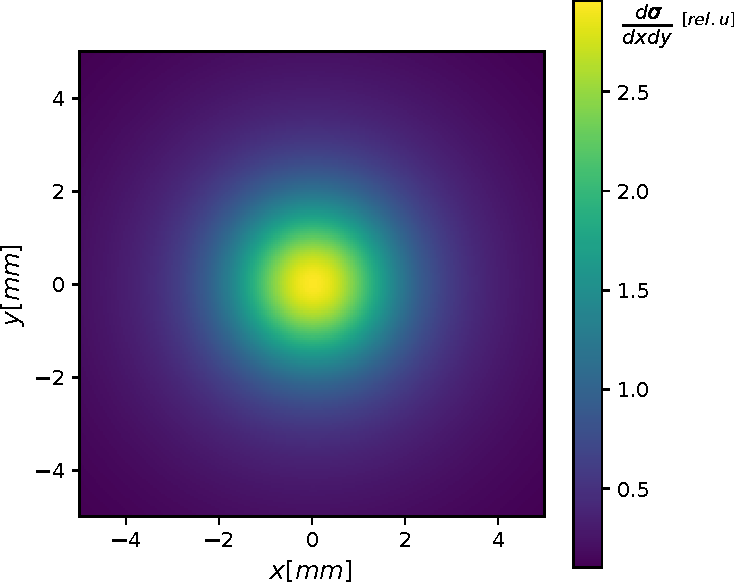
\includegraphics[width=1.\linewidth]{compton_dsdo_nopol.pdf}}
			\only<2>{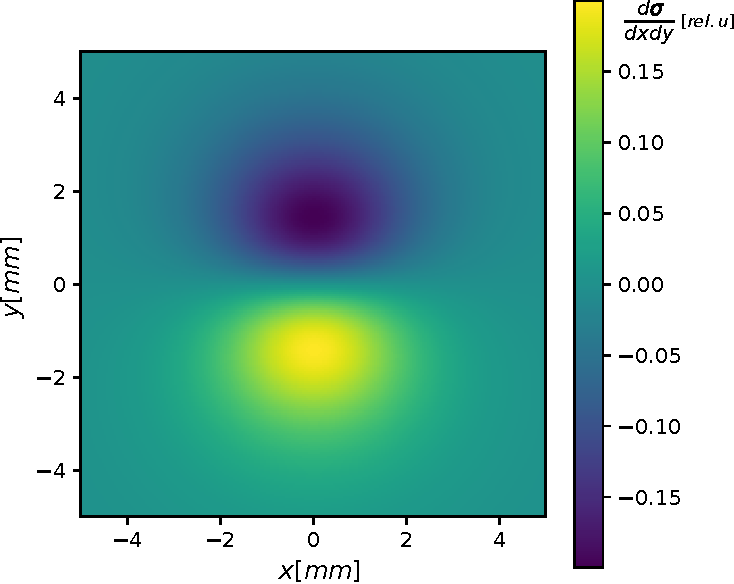
\includegraphics[width=1.\linewidth]{compton_dsdo_diff_v1.pdf}}
		\end{minipage} 
	\end{column}
\end{columns}
	\vfill
\footnotesize{*$\ell$ -- Расстояние от точки взаимодействия до точки регистрации рассеянного фотона, $\omega_0$ -- энергия лазерного фотона}
\end{frame}

\begin{frame}[t]
	\frametitle{Схема эксперимента по наблюдению поляризации}
	\begin{columns}
		\column{0.5\textwidth}
		\begin{minipage}[t][0.5\textheight]{\linewidth}
			\begin{itemize}
				\item Радиационная поляризация электронов 
				\item[$\Downarrow$]  Приготовление циркулярно поляризованных фотонов
				\item[$\Downarrow$] Рассеяние оптических фотонов на  пучке электронов
				\item[$\Downarrow$] Регистрация рассеянных $\gamma$ -- квантов с привязкой к поляризации начальных фотонов
				\item[$\Downarrow$] Получение координатных распределений для двух поляризаций.
			\end{itemize}
		\end{minipage}%
		\column{0.5\linewidth}
		\begin{minipage}[t][0.5\textheight]{\linewidth}
			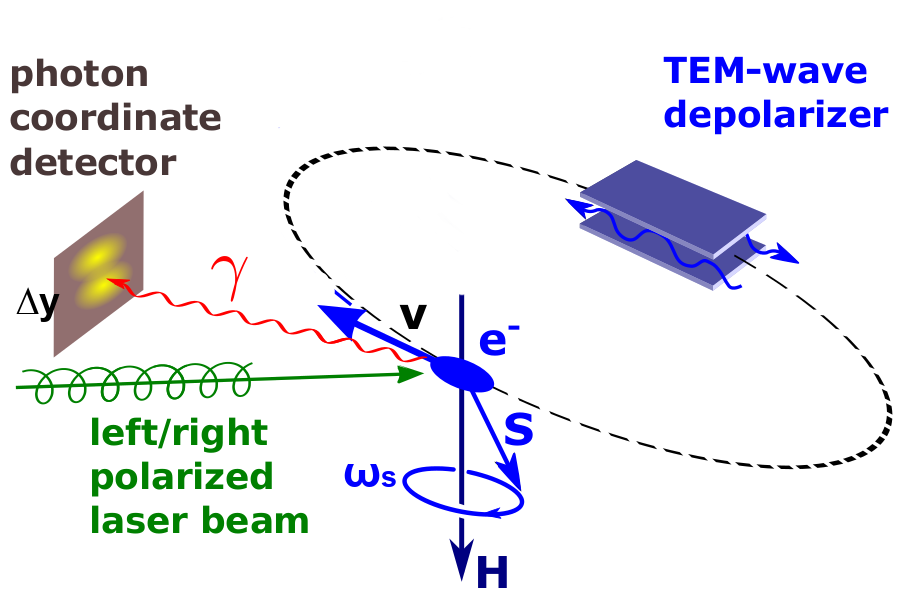
\includegraphics[width=1\linewidth]{mrd-lsrp.png}
		\end{minipage}%
	\end{columns}
	\begin{textblock*}{0.45\paperwidth}(0.65\paperwidth, 0.75\paperheight)
	\end{textblock*}
	
\end{frame}


\begin{frame}[t]
	\frametitle{Алгоритм измерения поляризации}
	\begin{itemize}
		\item[$\Downarrow$] Совместная аппроксимация распределений функциями вида:
		\begin{align*}
		F[L] &\sim \frac{d\sigma}{dxdy}\big(\sqrt{Q^2+U^2}, \varphi_0, P, +V \big) * G_2\big(\langle x\rangle, \langle y\rangle,\sigma_x, \sigma_y\big),\\
		F[R] &\sim \frac{d\sigma}{dxdy} \big(-\sqrt{Q^2+U^2}, \varphi_0, P, -V \big) * G_2\big(\langle x\rangle, \langle y\rangle,\sigma_x, \sigma_y\big).^*
		\end{align*}
		\item  Параметр P аппроксимирующей функции есть степень поляризации электронного пучка
	\end{itemize}
\flushleft
\footnotesize{*$G_2$ -- двумерная гауссова плотность распределения}	
\end{frame}

\begin{frame}[t]
	\frametitle{Валидация метода на MC моделировании}
	\begin{columns}
		\column{0.4\textwidth}
		\begin{minipage}[t][0.5\textheight]{\linewidth}
			\small
			\centering
			Параметры распределений: моделирования и его аппроксимации\\
			\vspace{0.5em}
			\begin{tabular}{|c||l|c|}
				\hline
				Параметр & MC & Fit \\
				\hline
				$\sqrt{Q^2+U^2}$ & 0.2 & $0.20 \pm 0.02$\\
				$V$ & 0.98 & $0.98 \pm 0.02$ \\
				$P$ & 0.9 & $0.89 \pm  0.11$ \\
				\hline
			\end{tabular}\\
		\flushleft
		Для оценок использовалась статистика:
		$N_{evt} = 5\cdot 10^5$\\
		Приведенное начение критерия Пирсона:
		$\chi^2/\text{ndf} = 0.82$
%			Параметры моделирования:
%			\begin{align*}
%				&N_{evt} = 5\cdot 10^5\\
%				&\xi_{lin} = 0.2\\ 
%				&V = 0.98\\
%				&P = 0.9
%			\end{align*}
%			Параметры из аппроксимации:
%			\begin{align*}
%			&\xi_{lin} = 0.20 \pm 0.02\\
%			&V = 0.98 \pm 0.02\\
%			&P = 0.89 \pm  0.11\\
%			&\chi^2/\text{ndf} = 0.82
%			\end{align*}%
		\end{minipage}%
		\column{0.6\linewidth}
		\begin{minipage}[t][0.5\textheight]{\linewidth}
			\only<1>{\centering\small{Координатное распределение для фотонов с левой циркулярностью}
				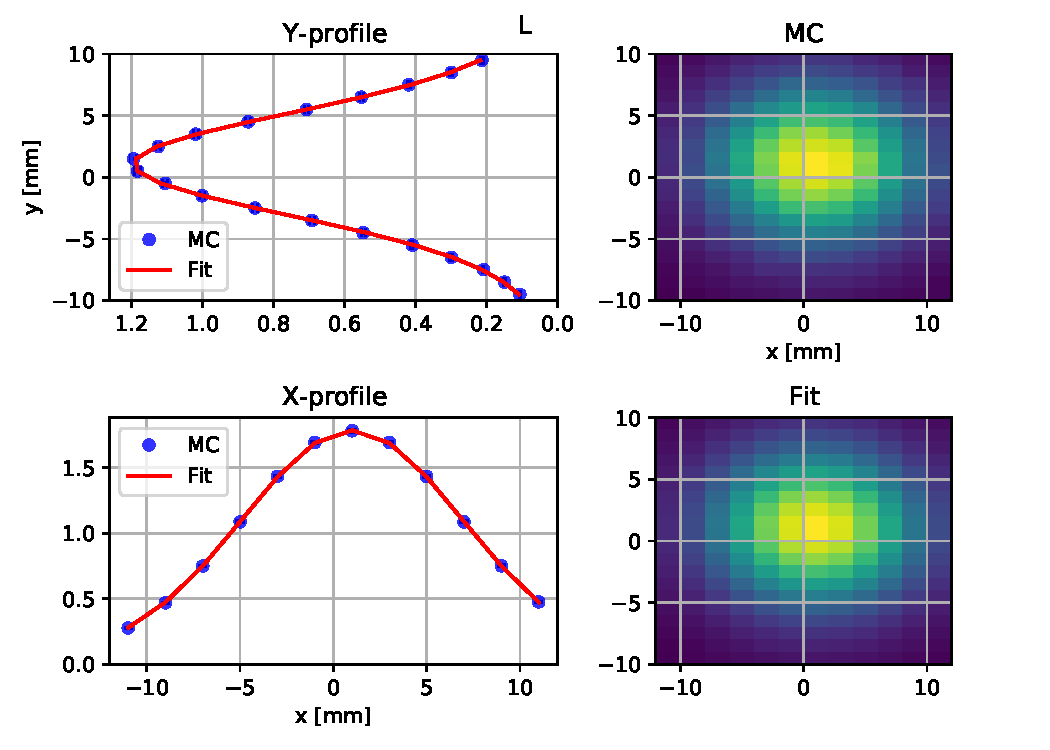
\includegraphics[width=1\linewidth]{MC_left.pdf}}
			\only<2>{\centering \small{Разностное распределение для фотонов с левой и правой циркулярностью }
				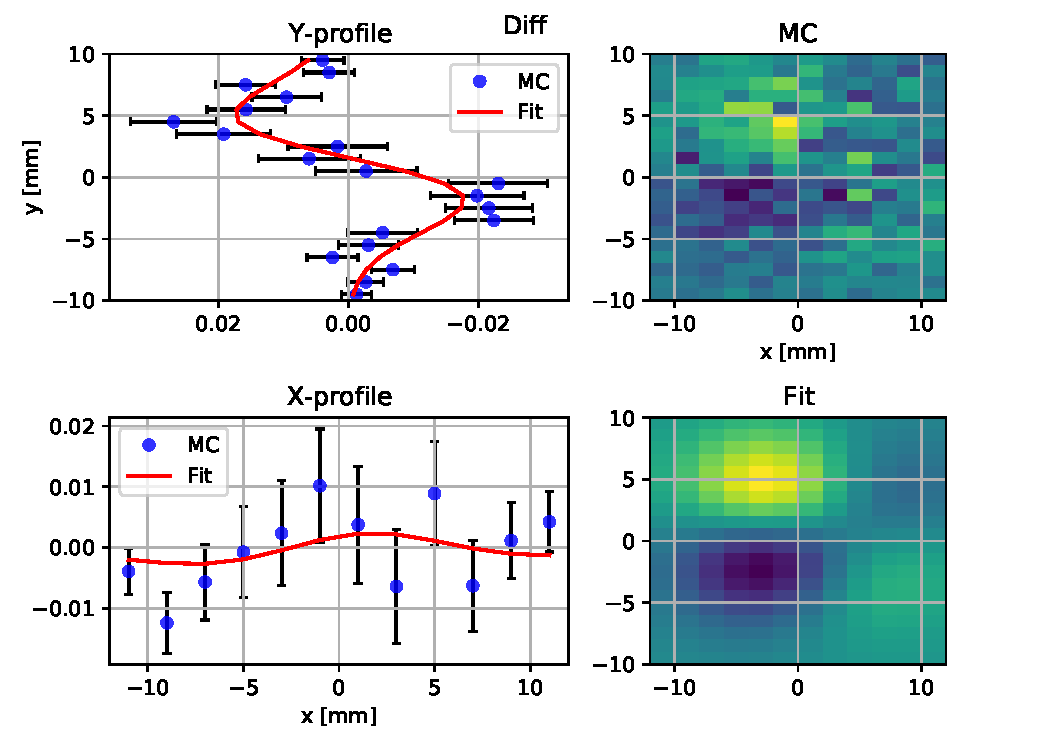
\includegraphics[width=1\linewidth]{MC_diff.pdf}}
		\end{minipage}%
	\end{columns}
	\begin{textblock*}{0.45\paperwidth}(0.65\paperwidth, 0.75\paperheight)
		%$\Delta \langle y \rangle = \cfrac{\omega_0}{2m_e}PL\Delta V$ 
	\end{textblock*}
\end{frame}

\begin{frame}[t]
	\frametitle{Оценка систематических ошибок метода}
	\begin{columns}
		\column{0.5\textwidth}
		\begin{minipage}[t][0.5\textheight]{\linewidth}
			\centering
			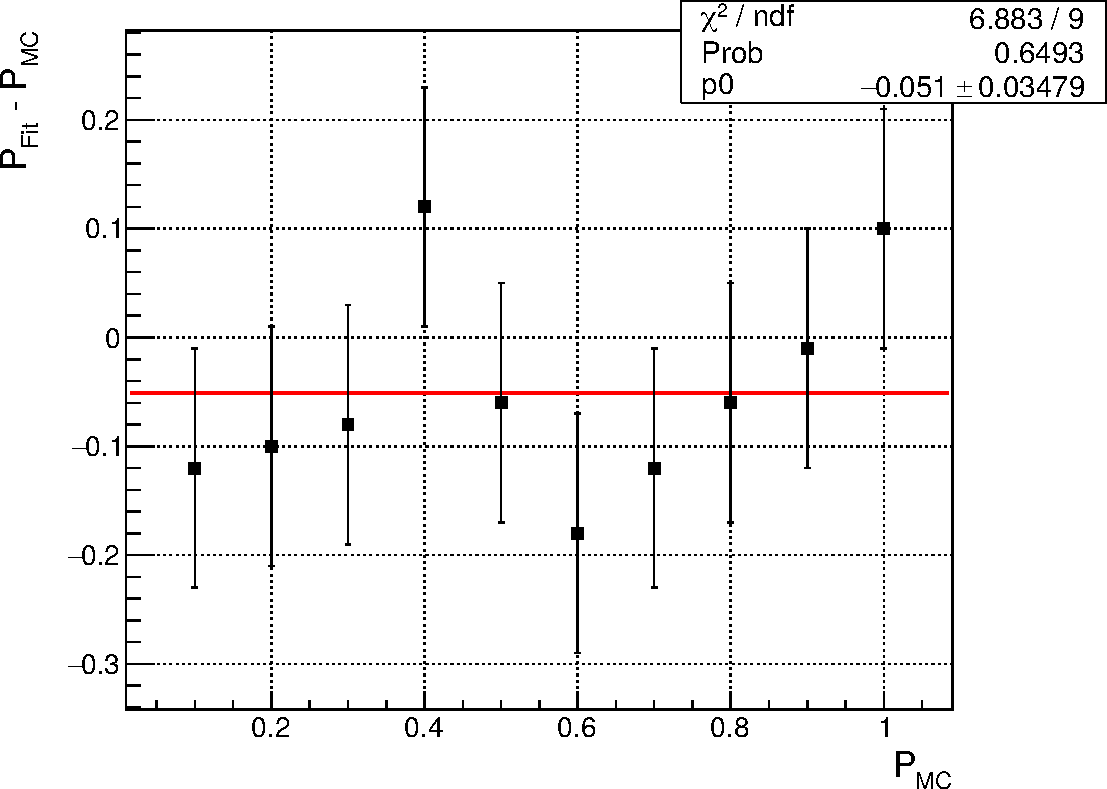
\includegraphics[width=1\linewidth]{MC_test.pdf}
			\footnotesize{Разность параметров поляризации пучка: заложенного в моделировании и определенного из аппроксимации}
		\end{minipage}%
		\column{0.5\linewidth}
		\begin{minipage}[t][0.5\textheight]{\linewidth}
			\centering
			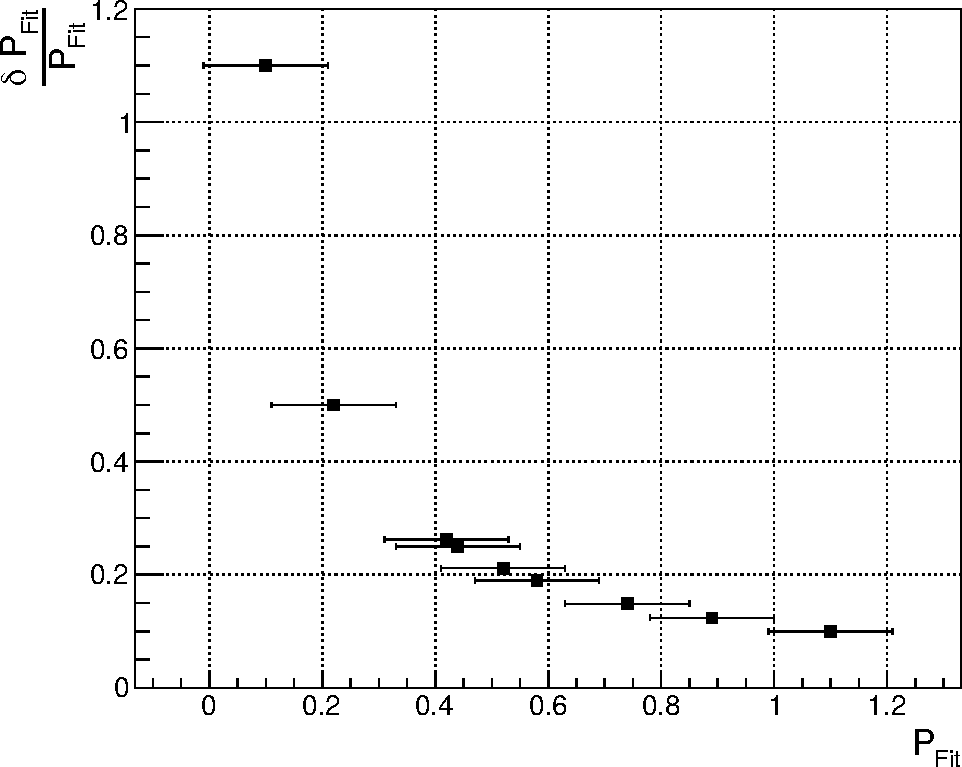
\includegraphics[width=0.9\linewidth]{MC_rel_error.pdf}
			\begin{tikzpicture}[remember picture,overlay]
			\path [thick,fill=calmGreen, opacity=0.3, draw=calmGreen, rounded corners=1ex] (-3.9,0.8) rectangle (-0.15,2);
			\end{tikzpicture}
			\footnotesize{Относительная ошибка определения поляризации электронного пучка}
		\end{minipage}%
	\end{columns}
	\end{frame}

\begin{frame}[plain]
	\centering
	\huge
	
	%\vspace{-0.3\paperheight}
	\begin{tcolorbox}[colframe=white, colback=calmBlue, width=0.8\paperwidth,
		arc=2.mm, boxsep=2mm,
		box align=center,
		halign=center,
		valign=center,
		]
		\Large
		\textcolor{white}{Экспериментальная реализация метода}	
	\end{tcolorbox}

\end{frame}
\begin{frame}[t]
	\frametitle{Принципиальная схема <<Лазерного поляриметра>>}
	\centering
	\begin{tikzpicture}
		\node[anchor=south west,inner sep=0] (image0) at (0,0){
			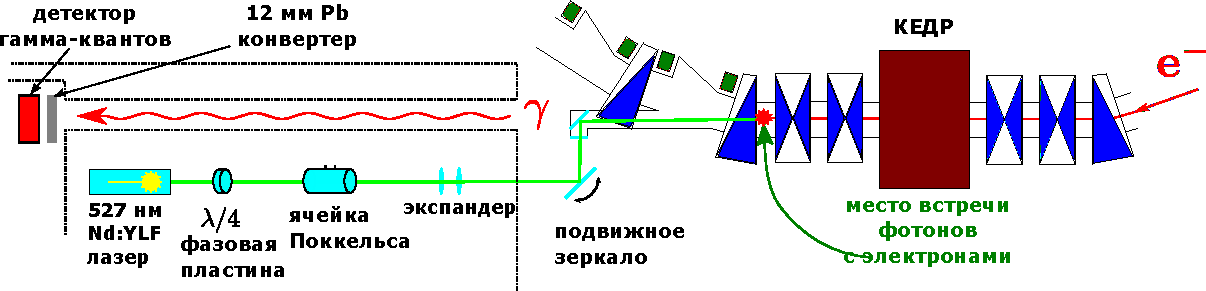
\includegraphics[width=0.8\linewidth]{LSRP_scheme}};
		\node[anchor=south west,inner sep=0] (image1) at (0,-3.5){
			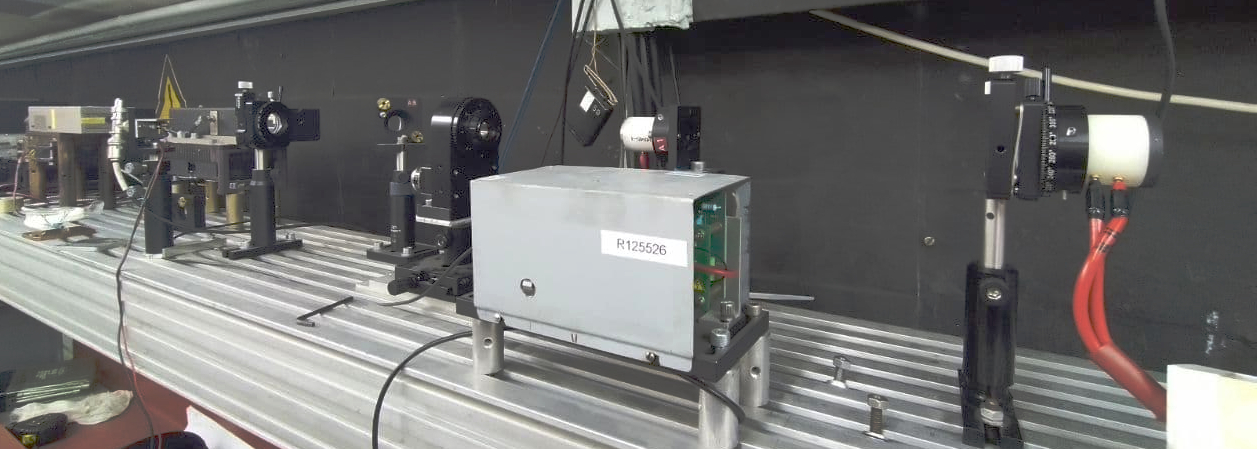
\includegraphics[width=0.6\linewidth]{optics_photo.jpg}};
		\node[anchor=south west,inner sep=0] (image2) at (9,-3.5){
			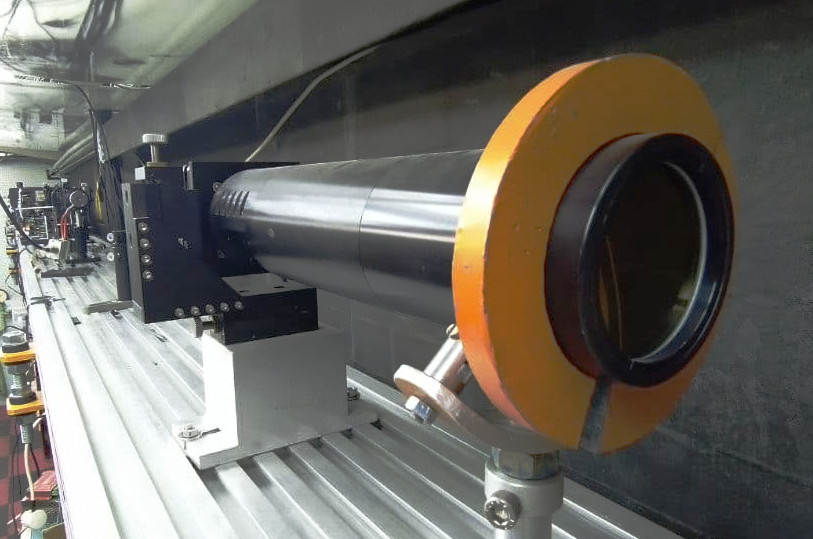
\includegraphics[width=0.325\linewidth]{telescope.jpg}};
		\draw[->,  -latex, ultra thick, calmBlue] (1.2,0.2) -- (0.4,-1);
		\draw[->,  -latex, ultra thick, calmBlue] (2.4,-0.) -- (3.3,-1);
		\draw[->,  -latex, ultra thick, calmBlue] (3.6,0.3) -- (4.7,-1.1);
		\draw[->,  -latex, ultra thick, calmBlue] (4.5,0.7) -- (11,-1.5);
			
	\end{tikzpicture}
\end{frame}
\begin{frame}[t]
	\frametitle{Проверка поляризации лазерного пучка}
	\centering
	\begin{tikzpicture}
	\only<1>{
		\node[anchor=south west,inner sep=0] (image3) at (1.5,0){
			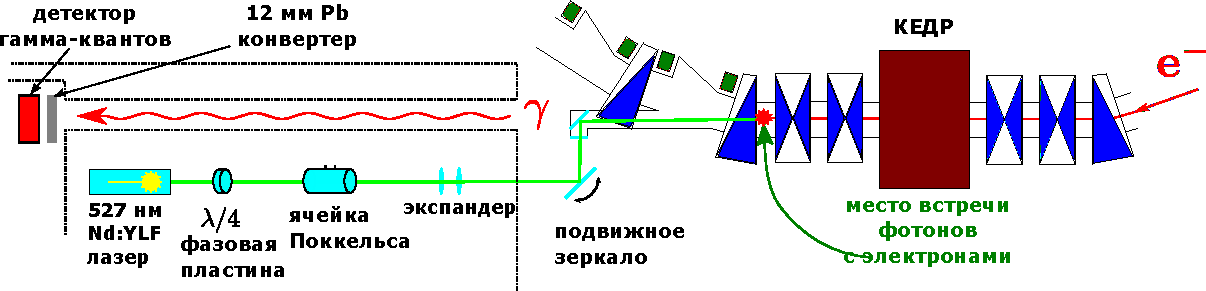
\includegraphics[width=0.8\linewidth]{LSRP_scheme}}};
	\only<2>{
		\node[anchor=south west,inner sep=0] (image4) at (1.5,0) {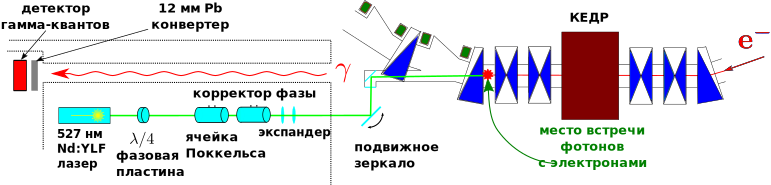
\includegraphics[width=0.8\linewidth]{LSRP_scheme_corr}};
	}	
	\only<1>{\node[anchor=south west,inner sep=0] (image2) at (7,-3.5){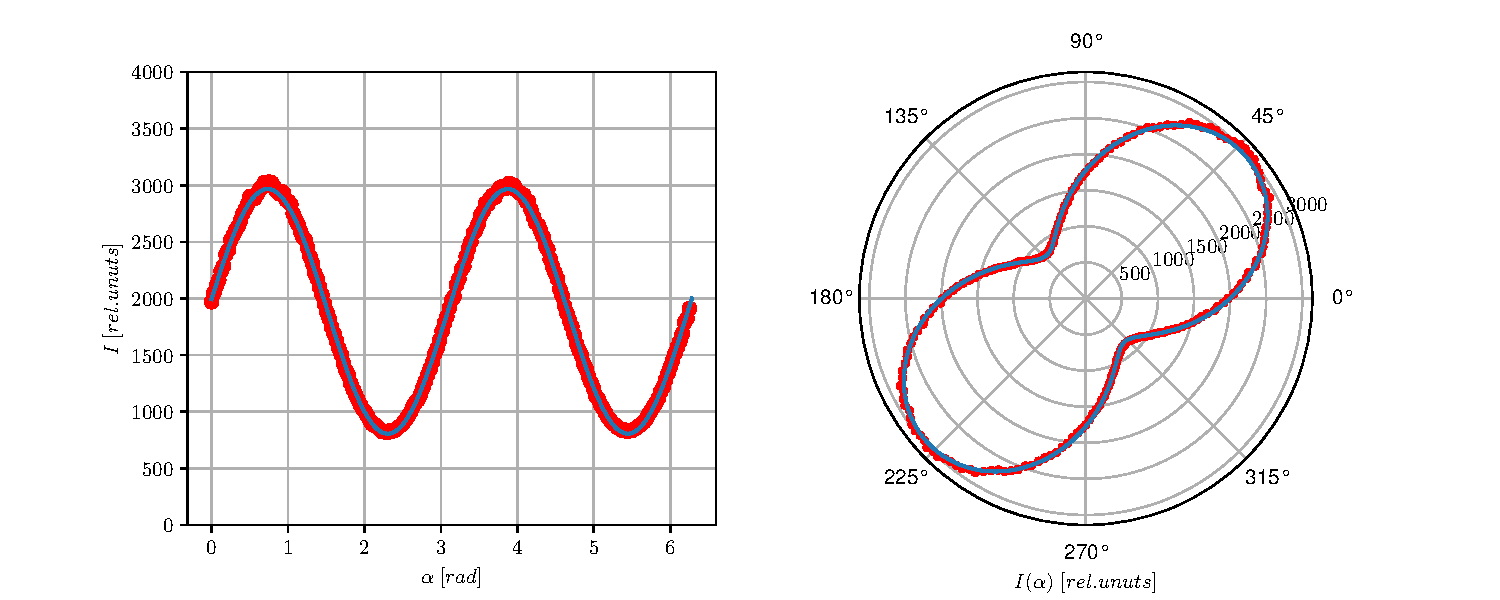
\includegraphics[width=0.6\linewidth]{I_plot_no_corr}};}
	\only<2>{\node[anchor=south west,inner sep=0] (image1) at (7,-3.5){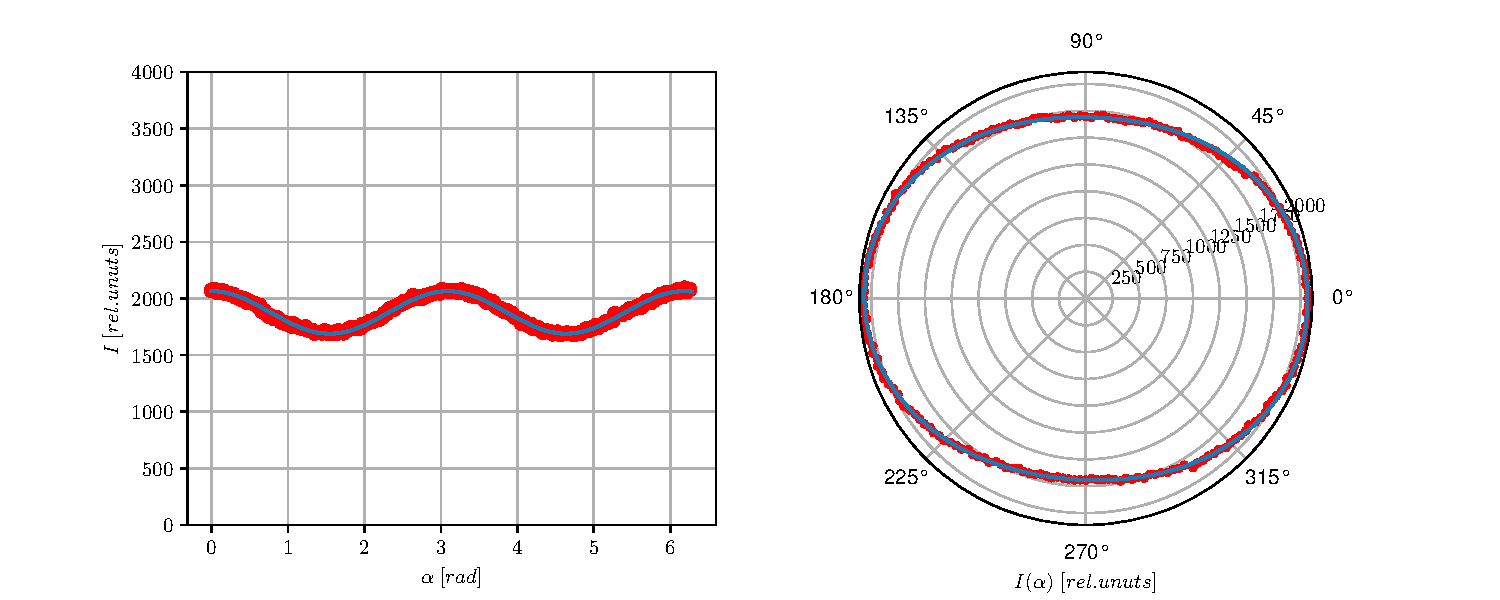
\includegraphics[width=0.6\linewidth]{I_plot_corr}};}
	
	%\draw[help lines,xstep=0.5,ystep=0.5] (-5,0) grid (5,10);
	%\node[draw,align=left,red] at (10.2,-1) {State of similarity};
	\draw[->,  -latex, ultra thick, calmRed] (9.7,-0.2) -- (7.4,1.7);
	\only<2>{\draw[->,  -latex, ultra thick, calmOrange] (5.5,2.5) -- (5.5,1.6);}
	\end{tikzpicture}\\
	\begin{textblock*}{0.4\paperwidth}(0.02\paperwidth, 0.45\paperheight)
		\flushleft \footnotesize Параметры поляризации после отражения от двух зеркал:
		\only<1>{
			\begin{align*}
			Q &= 0.44\pm0.01\\
			U &= 0.36\pm0.01\\
			V &= 0.82\pm0.01\\
			\sqrt{Q^2+U^2} &= \textcolor{calmRed}{0.57}\pm0.01
			\end{align*}%
		}
		\only<2>{
			\begin{align*}
			Q &= 0.10\pm0.01\\
			U &= 0.01\pm0.01\\
			V &= \textcolor{calmGreen}{0.99}\pm0.01\\
			\sqrt{Q^2+U^2} &= 0.10\pm0.01
			\end{align*}%
		}
	\end{textblock*}
\flushleft
\footnotesize{$Q,U,V$ -- параметры Стокса оптического пучка}
\end{frame}

\begin{frame}[t]
	\frametitle{Координатный детектор фотонов}
	\centering
	\begin{tikzpicture}
	\node[anchor=south west,inner sep=0] (image2) at (2,-3.5){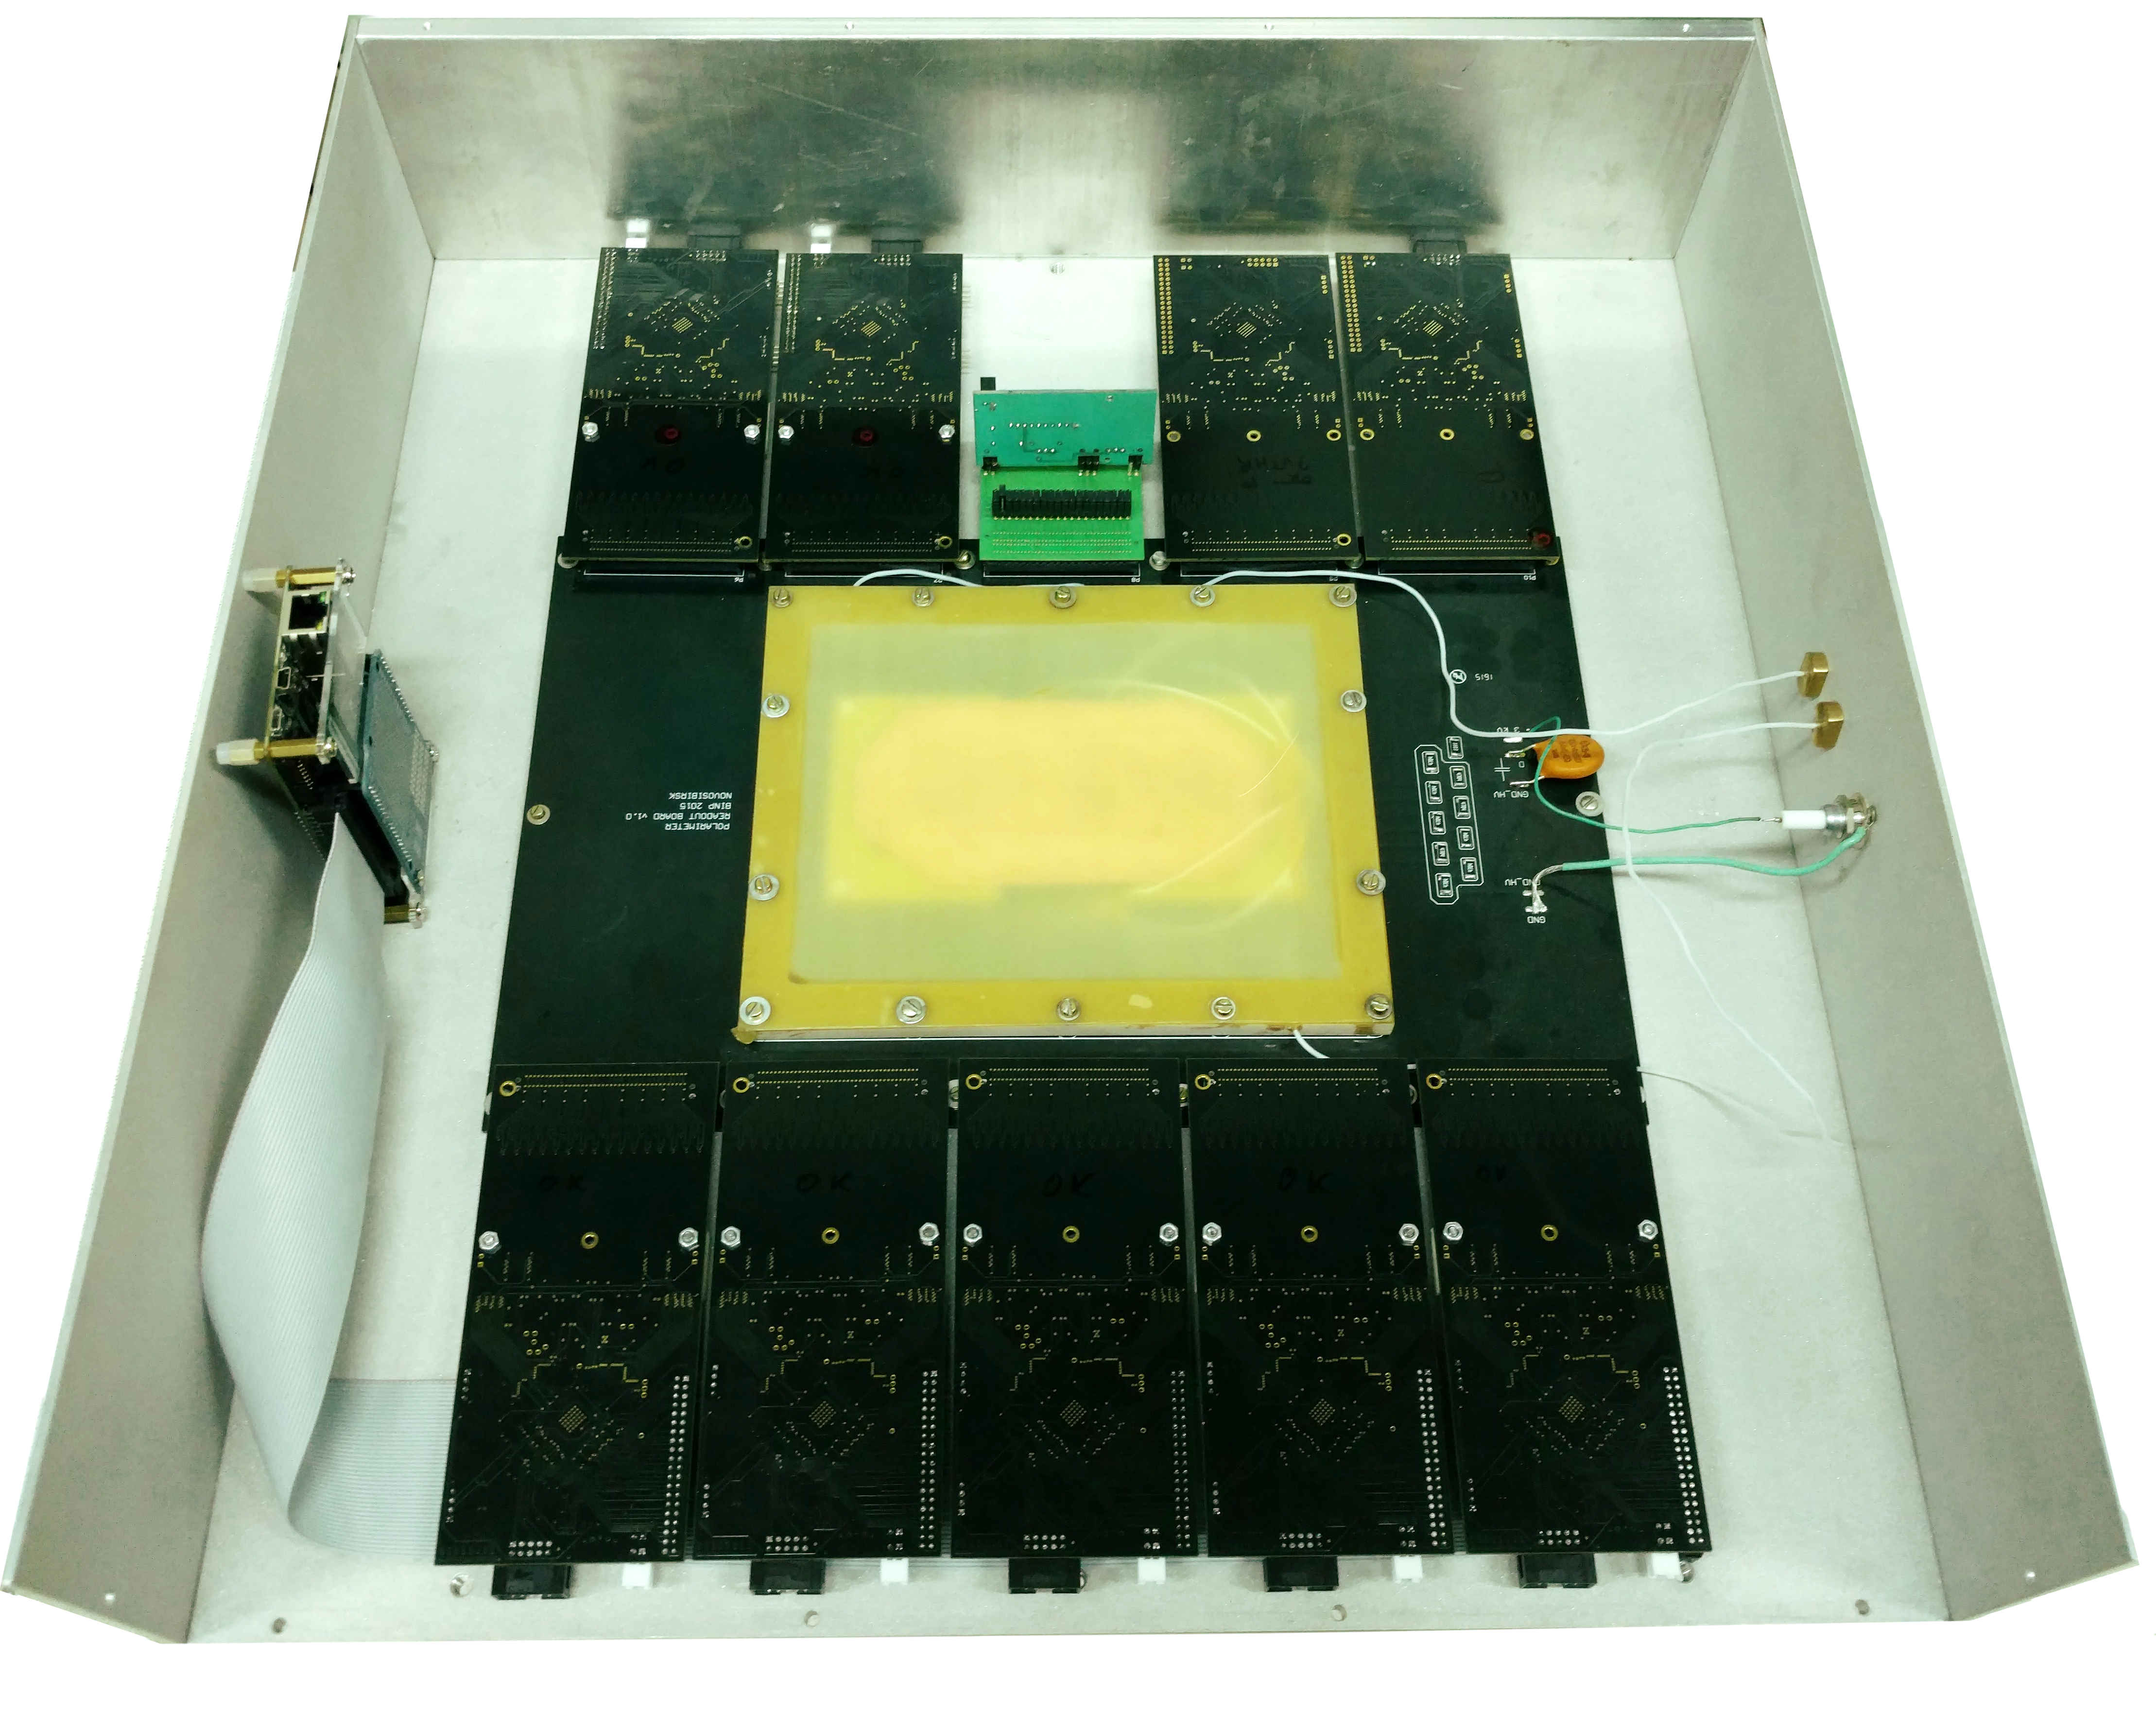
\includegraphics[width=0.25\linewidth]{GEM_prototype.jpg}};
	\node[anchor=south west,inner sep=0] (image3) at (7,-3.5){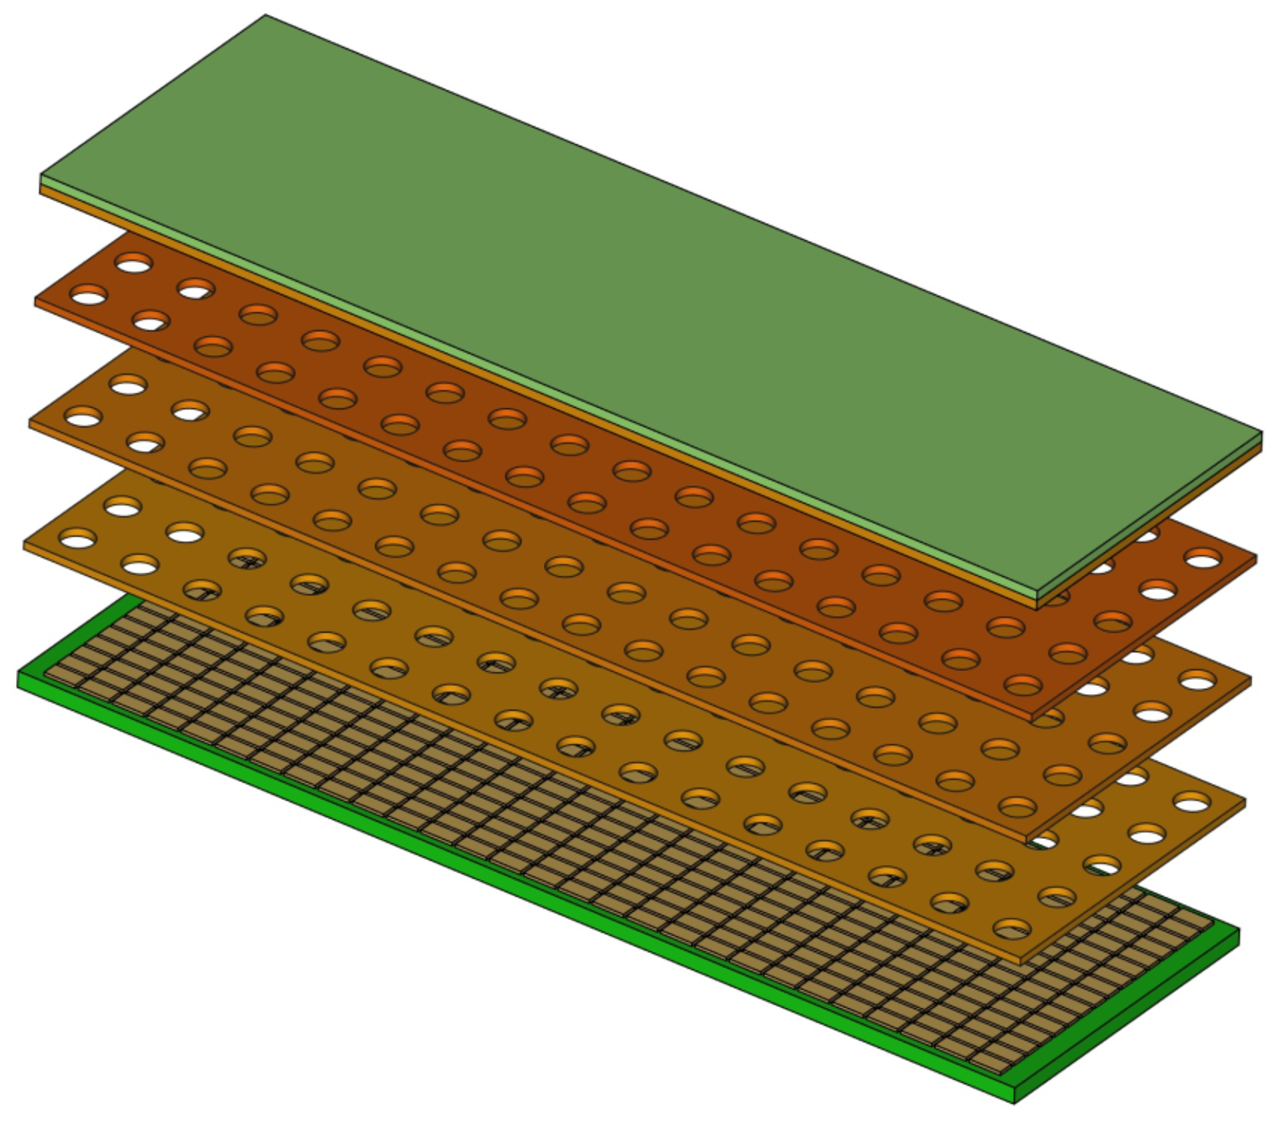
\includegraphics[width=0.25\linewidth]{GEM_model.pdf}};
		\draw[->,  -latex, ultra thick, calmRed] (image2) -- (image3);
		\node[black] at  (4.,-3.8) {\small{Прототип GEM детектора}};
		\node[black] at  (12.5,-1) {\small{Усиливающая}};
		\node[black] at  (12.5,-1.5) {\small{структура}};
		\draw[->,  -latex, ultra thick, calmRed] (11.8,-4) -- (10.7, -3.2);
		\draw[->,  -latex, ultra thick, calmRed] (12.6,-1.7) -- (10.8, -2.1);
	\end{tikzpicture}
	\begin{columns}
		\column{0.5\textwidth}
		\begin{minipage}[t][1.\textheight]{\linewidth}
			\vspace{0.5em}
			\begin{itemize}
				\small
				\item Усиливающая структура: 3 GEM электрода
				\item Чувствительная область: $40\times128$ мм
				\item Количество каналов: $640 + 512$ 
				\item Ожидаемые загрузки: $10-15$ кГц
			
			\end{itemize}
		\end{minipage}%
		\column{0.5\linewidth}
		\begin{minipage}[t][1.\textheight]{\linewidth}
			\centering
			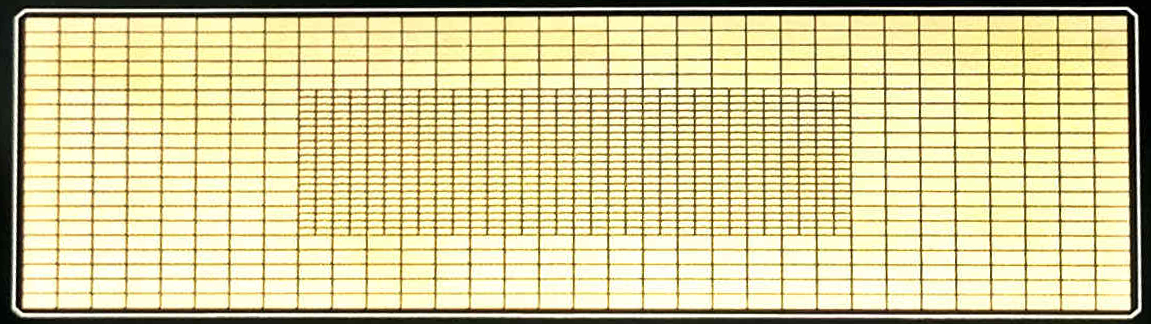
\includegraphics[width=0.8\linewidth]{Main_board_pads}\\
			\footnotesize{Считывающая структура}
			
		\end{minipage}%
	\end{columns}	
\end{frame}



\begin{frame}
	\frametitle{Методика проведения измерений}
	\begin{columns}
		\column{0.5\textwidth}
		\begin{minipage}[t][1.\textheight]{\linewidth}
			\vspace{1em}
			\begin{itemize}
				\onslide<1->{\item Сведение оптического пучка и пучка электронов}
				\onslide<2->{\item[$\Downarrow$] Поиск пятна рассеянных $\gamma$ -- квантов}
				\onslide<3->{\item[$\Downarrow$] Подстройка оптической поляризации по эффекту в детекторе}
				\onslide<4->{\item[$\Downarrow$] Накопление статистики и вычисление параметра поляризации пучка из аппроксимации данных}
			\end{itemize}
		\end{minipage}%
		\column{0.5\linewidth}
		\begin{minipage}[t][1.\textheight]{\linewidth}
			\only<2-3>{
				\centering 
				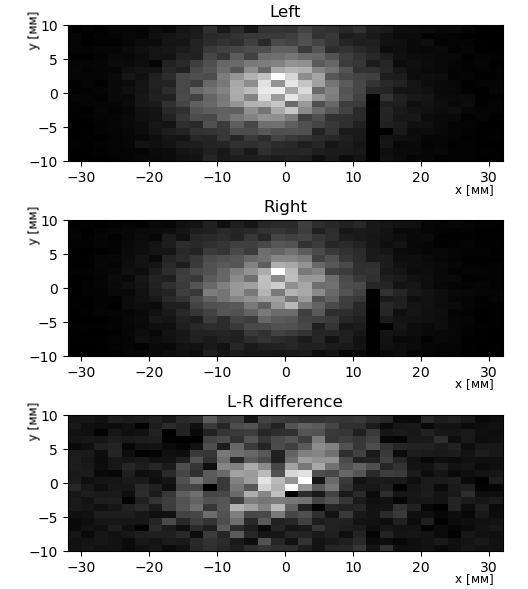
\includegraphics[width=0.7\linewidth]{Pol_preprocess_monitor.png}\\
				\footnotesize{Монитор детектора: по нему осуществлялись первичный контроль и настройка системы}
			}
		\only<4>{
			\centering 
			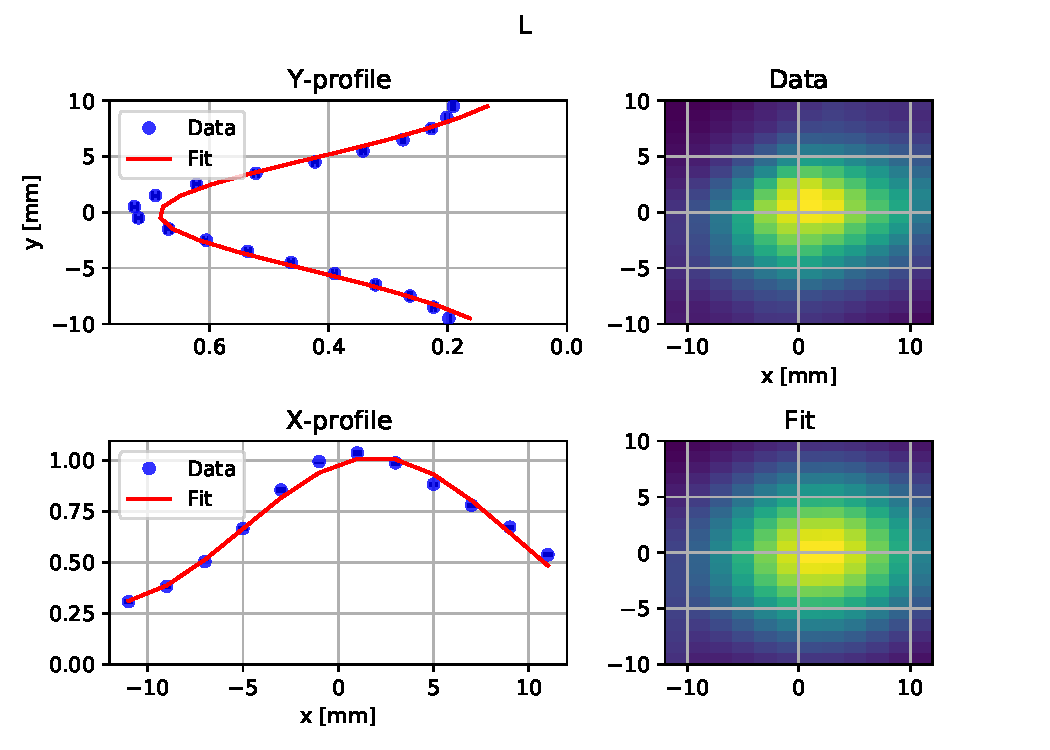
\includegraphics[width=1\linewidth]{data_fit_L_P063-014_Q053-003_V085-003.pdf}\\
			\footnotesize{Аппроксимация данных с детектора теоретической плотностью распределения}
		}
		
		\end{minipage}%
	\end{columns}	
\end{frame}
\begin{frame}[t]
	\frametitle{Результаты: измерение поляризации электронного пучка}
	\begin{columns}
		\column{0.5\textwidth}
		\begin{minipage}[t][1.\textheight]{\linewidth}
			\begin{itemize}
				\item[$\checkmark$] Смогли наблюдать поляризацию
				\item[$\checkmark$] Из аппроксимации данных:
					\begin{tabular}{|c|c|}
					\hline
					Параметр & Значение \\
					\hline
					$\sqrt{Q^2+U^2}$ &  \textcolor{calmOrange}{$0.53 \pm 0.02$}\\
					$V$ &  $0.85 \pm 0.03$ \\
					$P$ &   \textcolor{calmGreen}{$0.63 \pm  0.14$}\\
					\hline
				\end{tabular}\\
				\item В этой точке предсказывалась поляризация $P_{th} > 0.8$
				\item[$\Rightarrow$] Необходимо улучшать точность настройки оптической поляризации
				\item[$\Rightarrow$] А также изучить детекторные систематики
			\end{itemize}
		\end{minipage}%
		\column{0.5\linewidth}
		\begin{minipage}[t][1.\textheight]{\linewidth}
			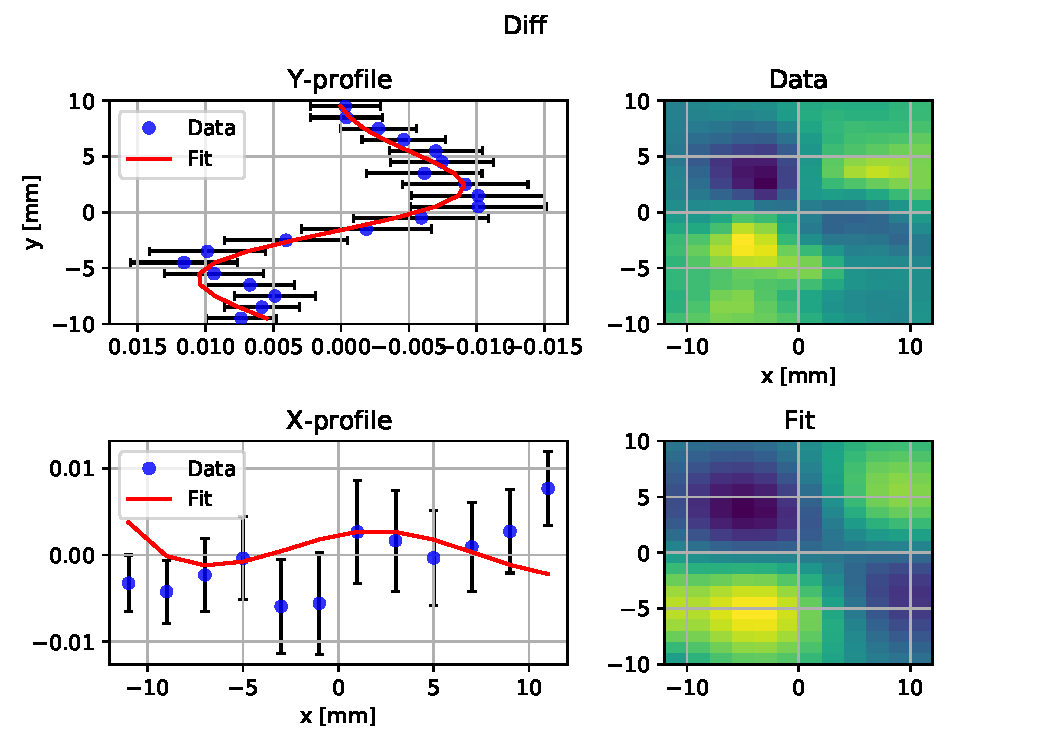
\includegraphics[width=1\linewidth]{data_fit_diff_P063-014_Q053-003_V085-003.pdf}
			\footnotesize{Аппроксимация разностного распределения данных}
		\end{minipage}%
	\end{columns}	
\end{frame}

\begin{frame}[t]
	\frametitle{Результаты: сканирование по энергии в точке $E\approx 4.1$ GeV}
	\begin{columns}
		\column{0.4\textwidth}
		\begin{minipage}[t][0.8\textheight]{\linewidth}
			\begin{itemize}
				\item Использовали метод резонансной деполяризации
				\item Измерили энергию пучка в точке $E\approx 4.1$ GeV
				\item[$\checkmark$]$E_{exp} = 4116\pm0.15$  Mev ($\delta E/E \sim 10^-5$)
				\item Отработали методику
			\end{itemize}
		\end{minipage}%
		\column{0.6\linewidth}
		\begin{minipage}[t][1.\textheight]{\linewidth}
			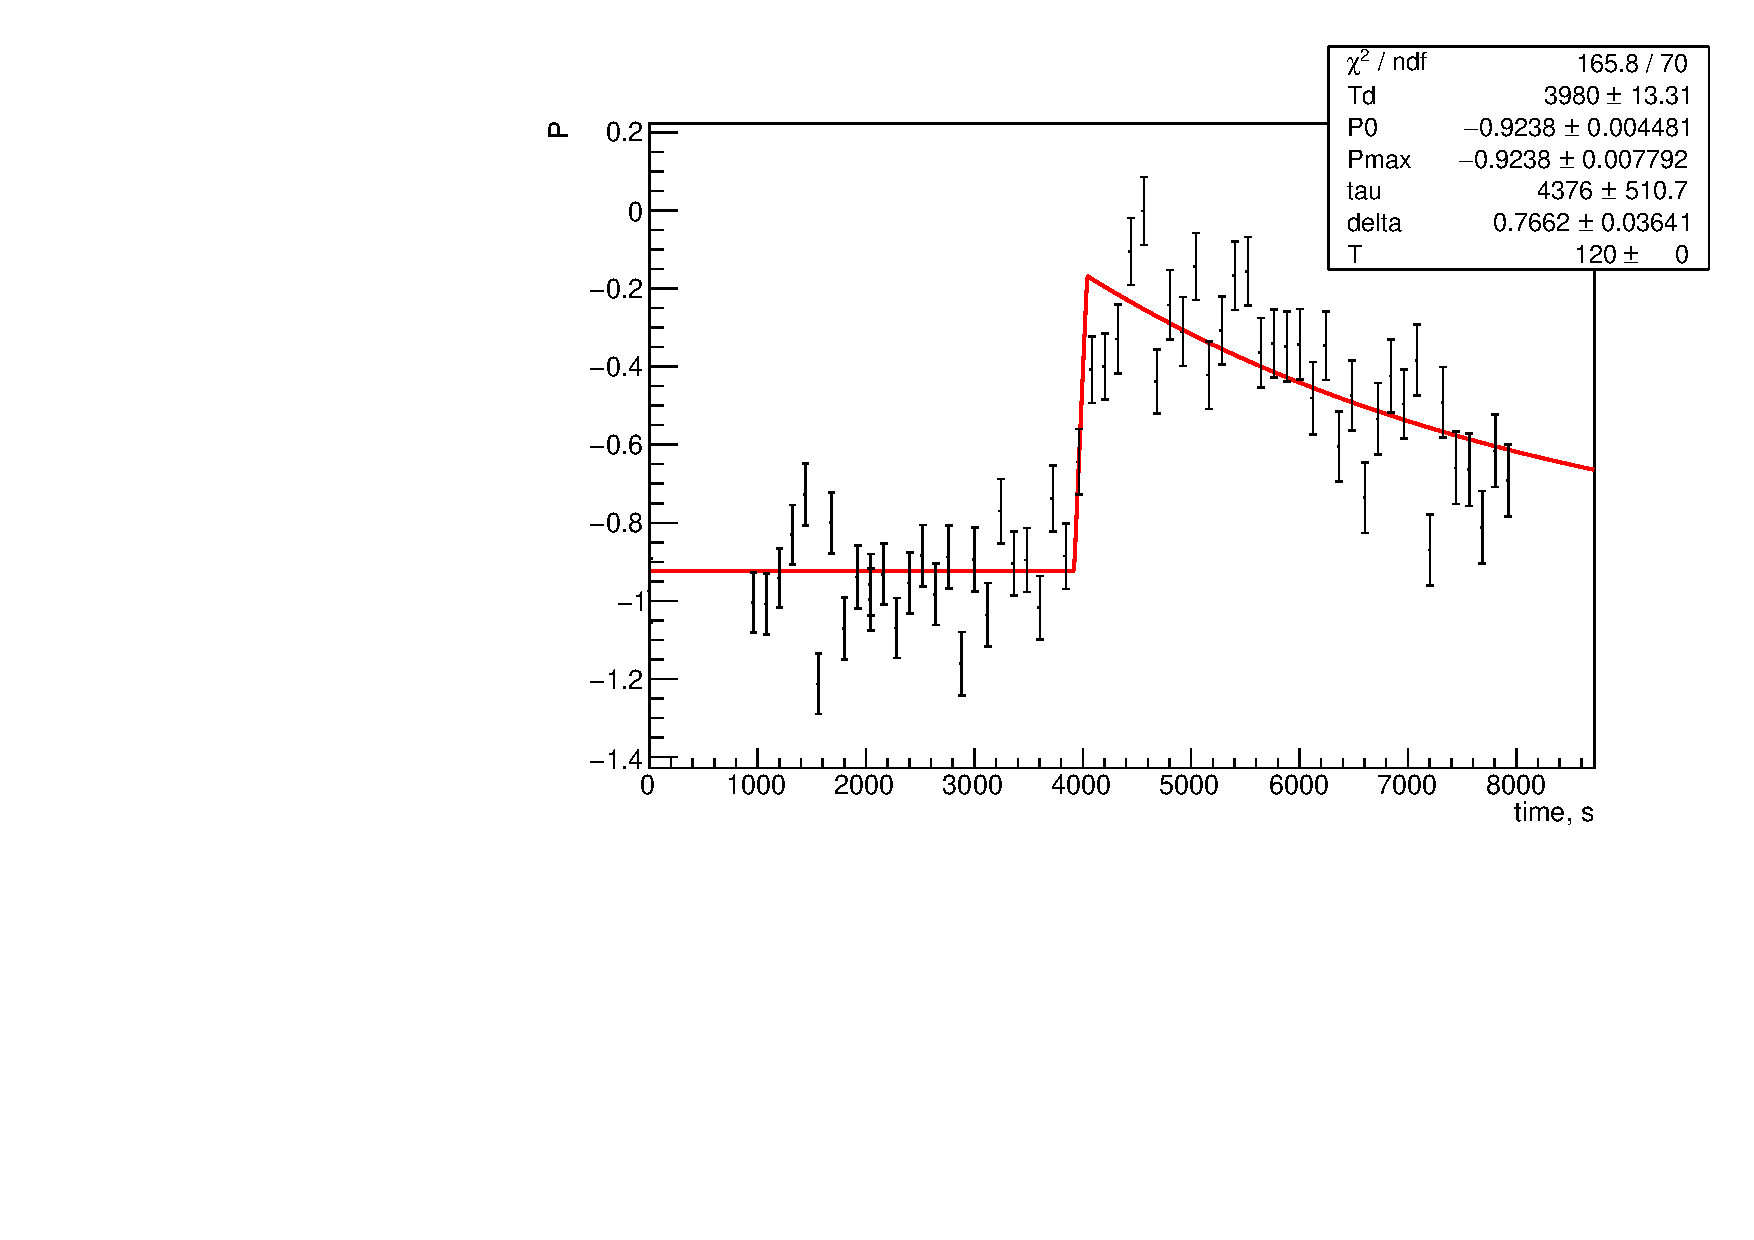
\includegraphics[width=1\linewidth]{jump1.pdf}
			\footnotesize{Сканирование по частоте деполяризующего поля. За привязку значения времени к энергии отвечает параметр Td}
		\end{minipage}%
	\end{columns}	
\end{frame}








\begin{frame}[t]
	\frametitle{Заключение}
	\begin{itemize}
		\item  Создан прототип <<Лазерного поляриметра>> --- ключевая часть новой системы измерения энергии ускорителя ВЭПП-4Мы
		\item Проведен обзор теории рассеяния поляризованных фотонов на электронах
		\item Разработано программное решение для обработки и анализа данных с координатного детектора $\gamma$ -- квантов
		\item[\textcolor{calmGreen}{$\checkmark$}] На Монте-Карло моделировании оценены систематики метода аппроксимации ($\delta P \sim 5\%$)
		\item[\textcolor{calmGreen}{$\checkmark$}] Измерена поляризация электронного пучка: $P = 0.63 \pm 0.14\pm 0.05$ \% 
		\item[\textcolor{calmGreen}{$\checkmark \checkmark$}] Проведено первое сканирование энергии с использованием новой системы $\delta E/E \sim 10^{-5}$!
	\end{itemize}
\end{frame}

\maketitle


\backupbegin
%\begin{frame}[t]
%\frametitle{Схема <<Лазерного поляриметра>>}
%\centering 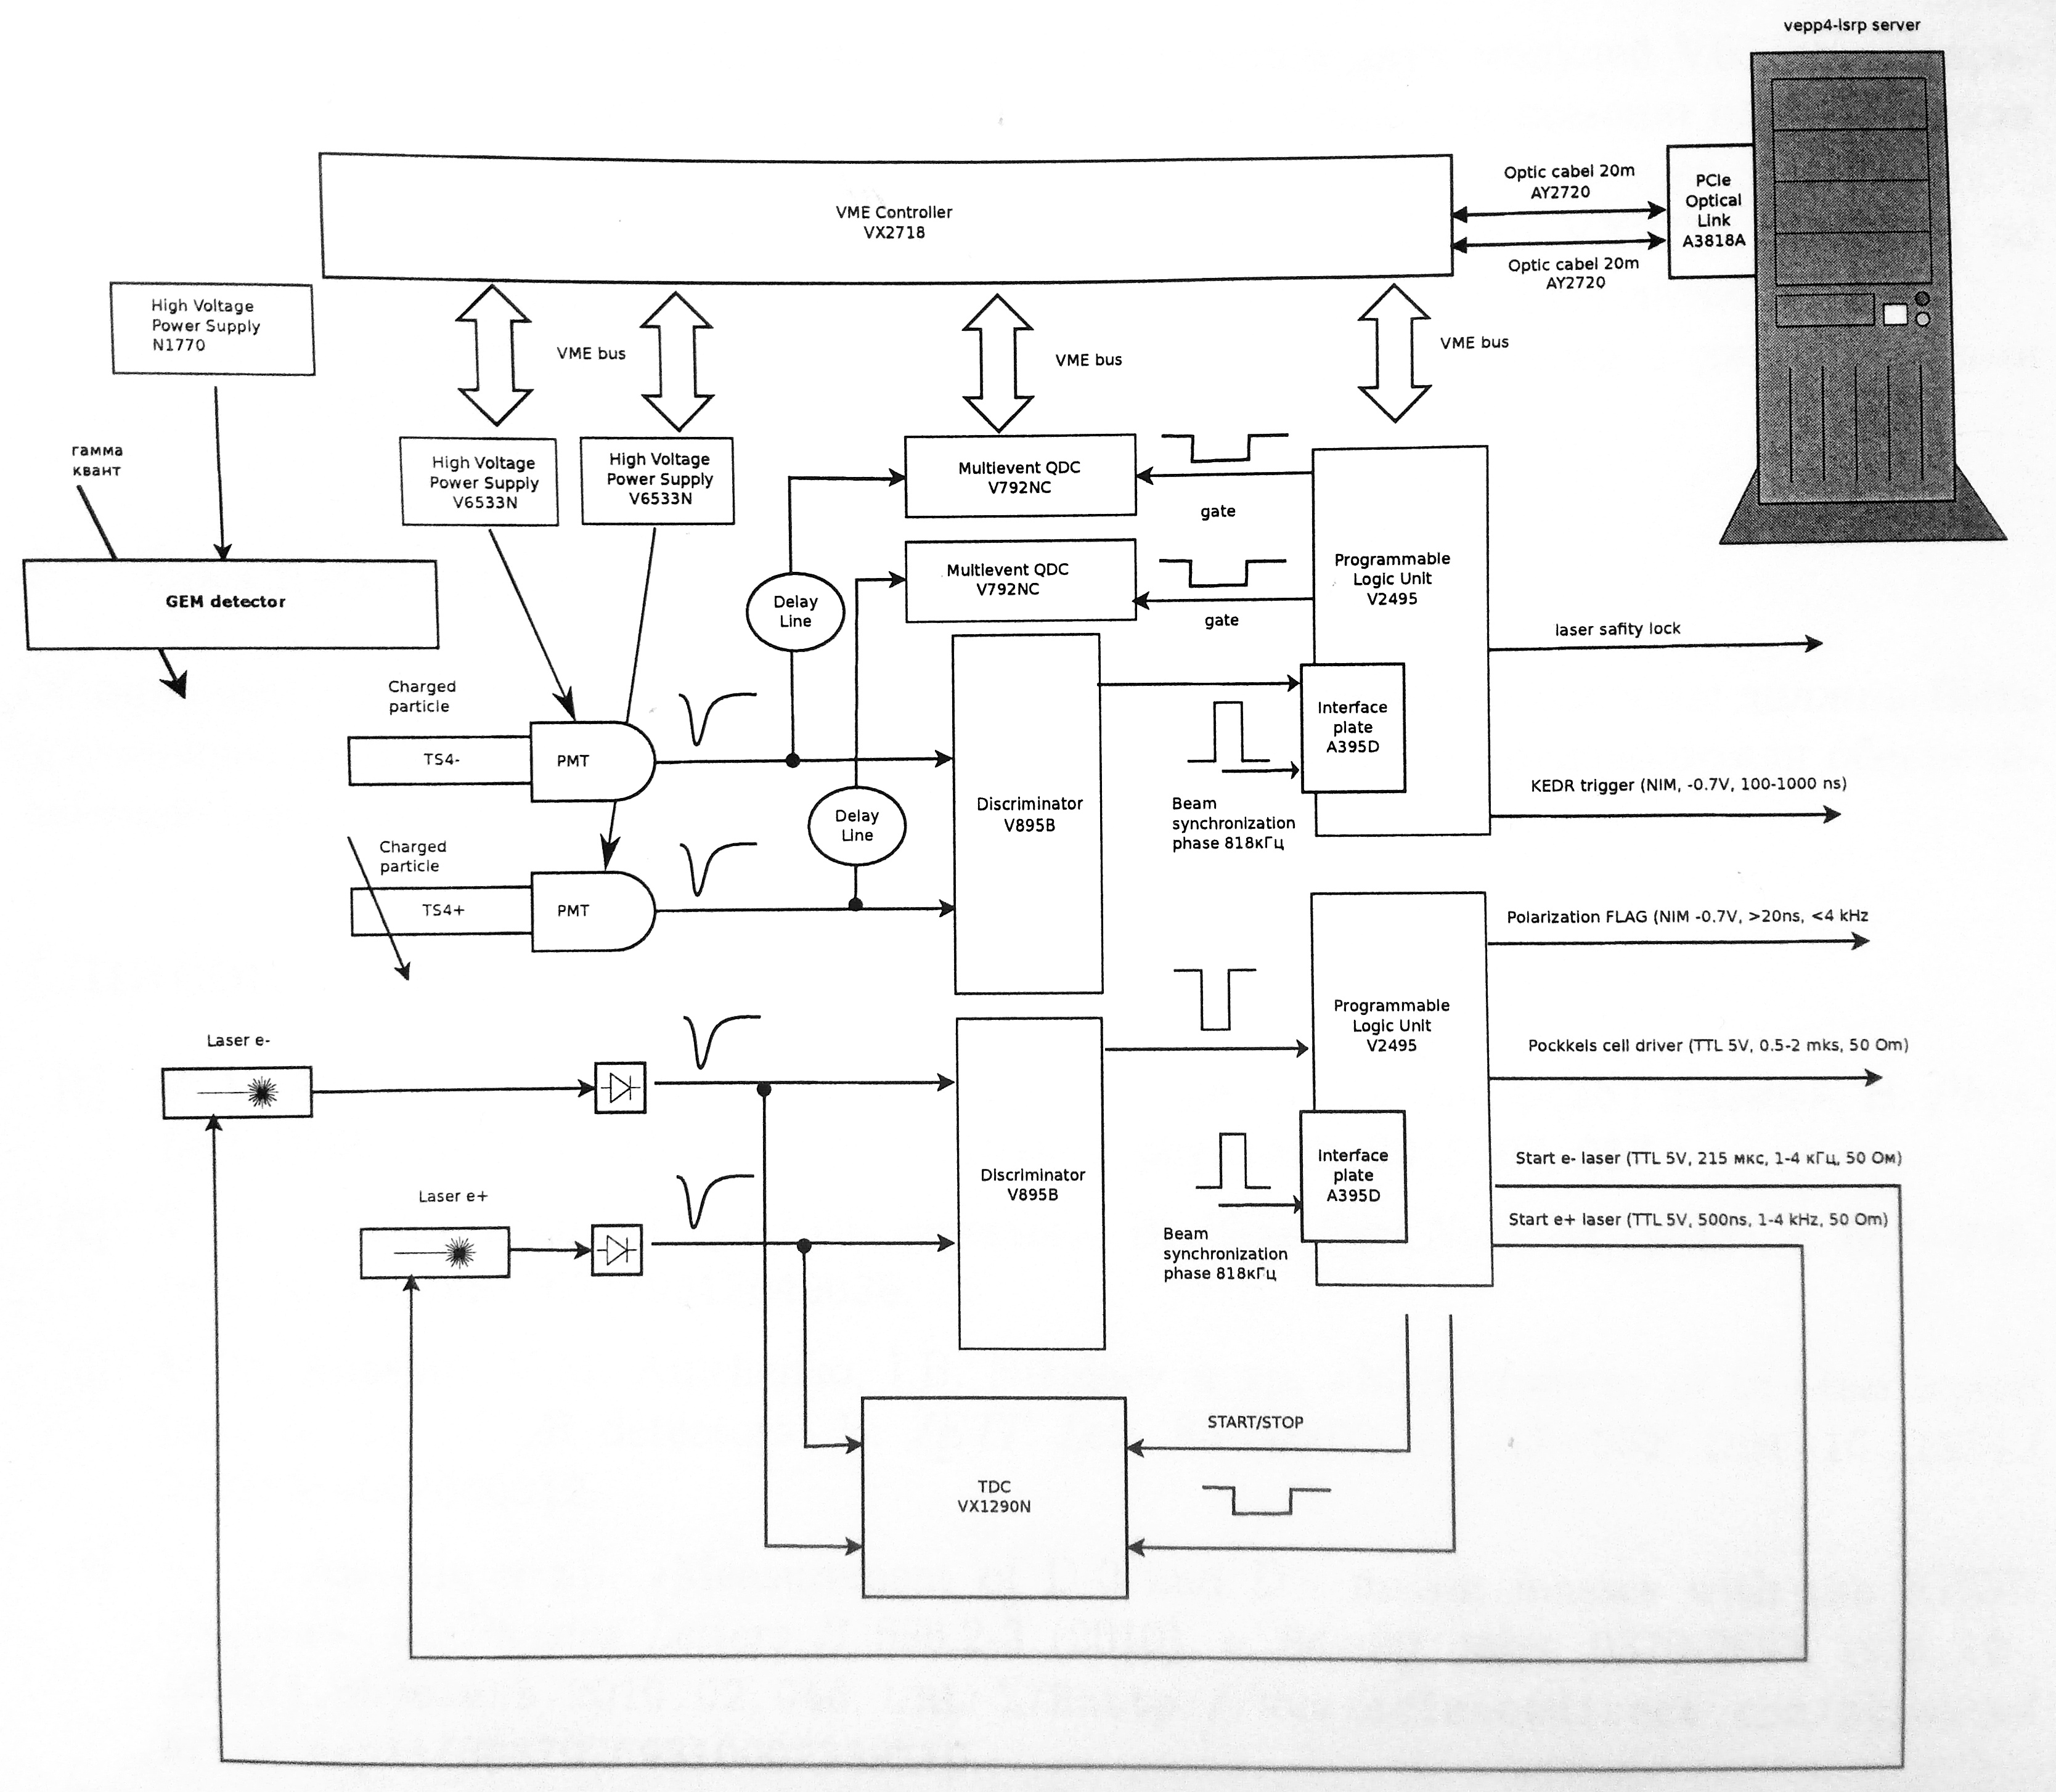
\includegraphics[width=0.65\linewidth]{DAC_scheme.jpg}
%\end{frame}
%
%\begin{frame}[t]
%\frametitle{Крейт и основные блоки уже установлены}
%\centering 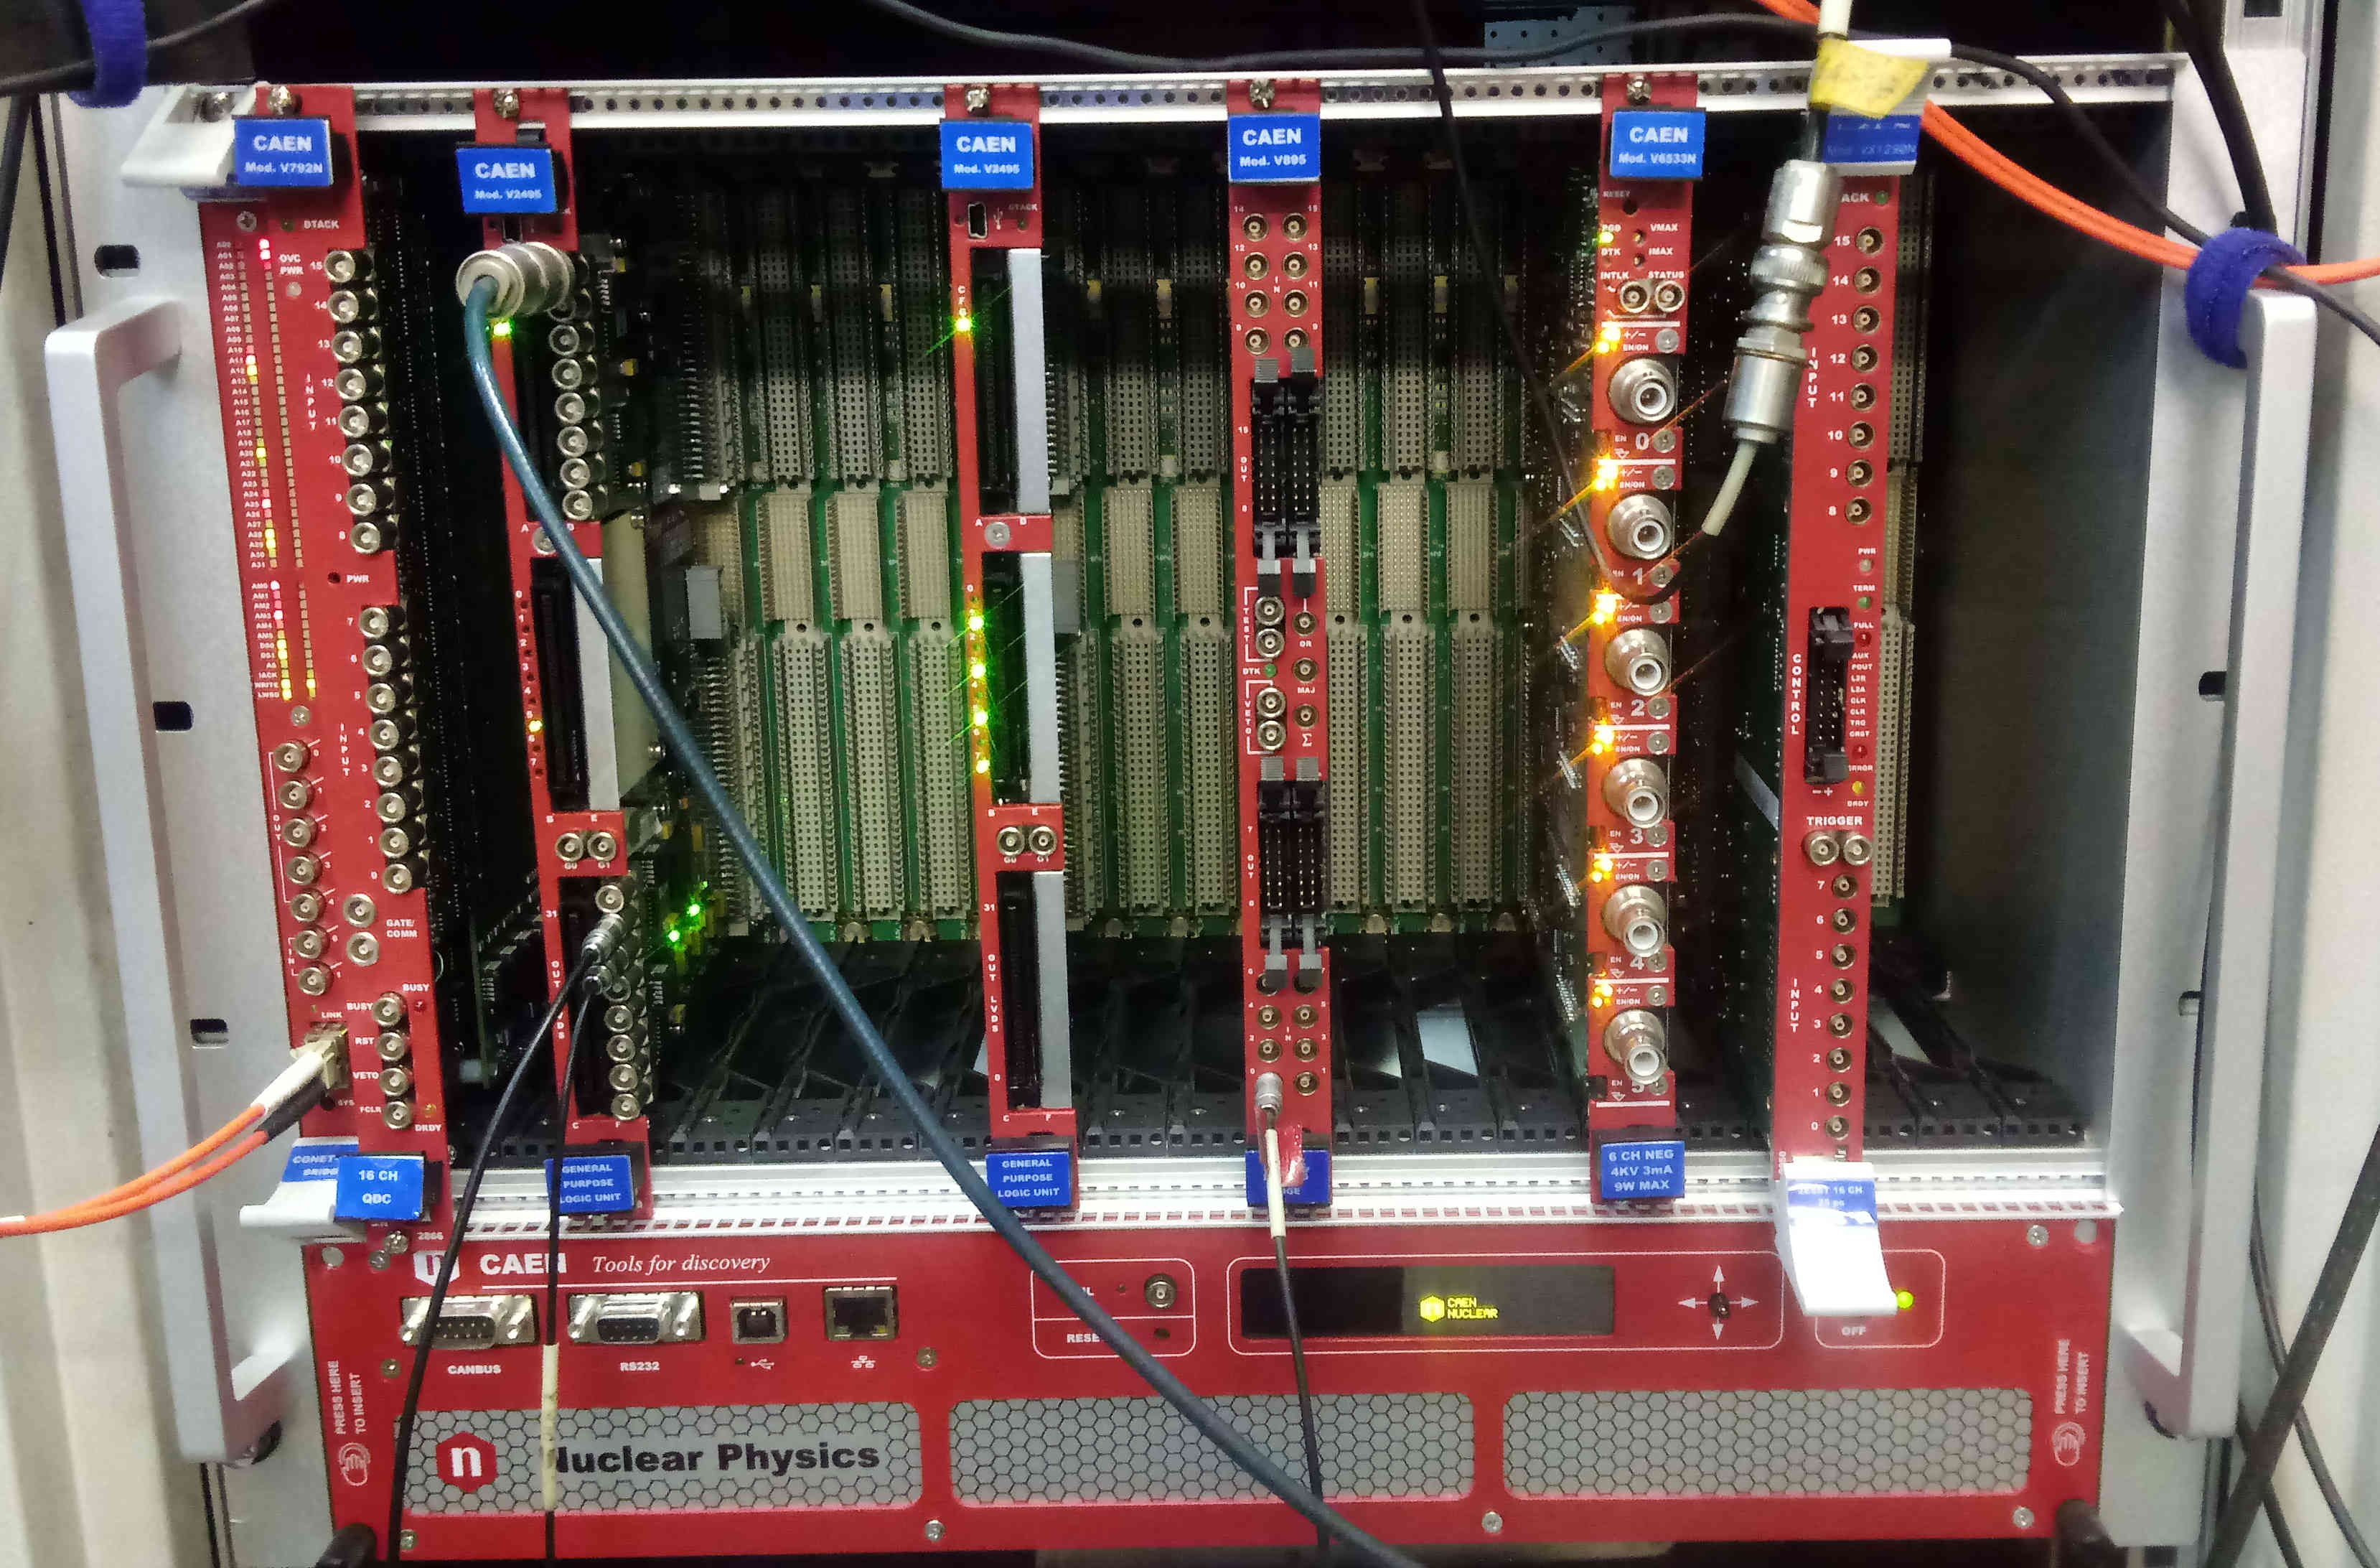
\includegraphics[width=0.8\linewidth]{CAEN_VME.jpg}
%\end{frame}

\begin{frame}[t]
	\frametitle{Backup: Метод резонансной деполяризации}
	\begin{columns}
		\column{0.5\textwidth}
		\begin{minipage}[t][0.5\textheight]{\linewidth}
			\begin{itemize}
				\item Радиационная поляризация пучков: 
				$P = G \zeta{_0}(1-e^{-t/G\tau_p})$
				\item Воздействие деполяризующим полем:
				$\omega_s=  k\omega_{r} \pm \textcolor{calmRed}{\omega_d}$
				\item Энергию находим из соотношения частот:
				$\omega_s=  \omega_{r}\bigg(\cfrac{q'}{q_0}\cfrac{\textcolor{calmRed}{E}}{mc^2}+1\bigg)$
			\end{itemize}
		\end{minipage}%
		\column{0.5\linewidth}
		\begin{minipage}[t][0.5\textheight]{\linewidth}
			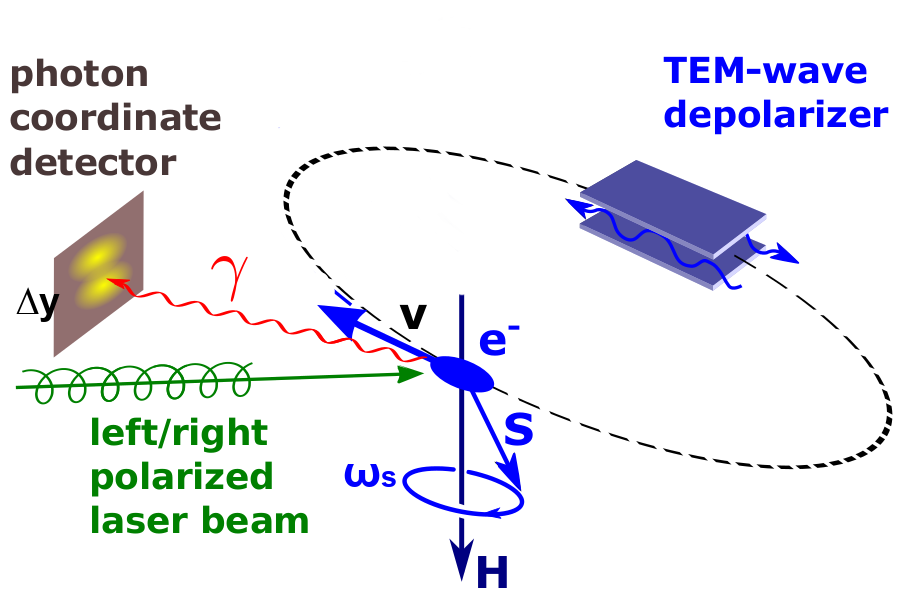
\includegraphics[width=1\linewidth]{mrd-lsrp.png}
		\end{minipage}%
	\end{columns}
	\begin{textblock*}{0.45\paperwidth}(0.65\paperwidth, 0.75\paperheight)
		$\Delta \langle y \rangle = \cfrac{\hbar\omega_0}{2m_e c^2}P\ell\Delta V$ 
	\end{textblock*}
	
\end{frame}

\begin{frame}[t]
\frametitle{Backup: Основные систематики измерений}
	\begin{itemize}
	\item[$\checkmark$]Асимметрия флагов поляризации\\ \textcolor{calmGreen}{(Контролируется аппаратно)}
	\item[$\checkmark$] Нециркулярность лазерного пучка \\
	\textcolor{calmGreen}{(Измерили и теперь можем корректировать)}
	\item[$\Rightarrow$] Неоднородность эффективности регистрации детектора \\
	\textcolor{calmRed}{(Ждем пока заработает весь детектор)}
	\item[$\checkmark$] Дрейф орбиты пучка \\
	\textcolor{calmGreen}{(Наблюдаем и можем нивелировать)}
\end{itemize}
\end{frame}

\begin{frame}
	\frametitle{Backup: Обзор существующих методов измерения $E$}
	\begin{columns}[T]
		\begin{column}{0.32\linewidth}
			\begin{minipage}{1.\linewidth}
				\centering
				Через $B$ методом ЯМР\\
				$\cfrac{\textcolor{calmRed}{p}c}{eB} = R$
				\small
				\begin{itemize}
					\item[\textcolor{calmGreen}{\checkmark}] Простой метод контроля E
					\item[\textcolor{calmRed}{$\times$}] Измерение локально
					\item[\textcolor{calmRed}{$\times$}] Низкая точность ($\delta E/E \sim 10^{-3}$)
				\end{itemize}
			\end{minipage}
		\end{column}
		\begin{column}{.01\linewidth}
			\rule{.1mm}{.8\textheight}
		\end{column}
		\begin{column}{0.32\linewidth}
			\begin{minipage}{1.\linewidth}
				\centering
				По энергии ОКР фотонов\\
				\small
				\vspace{1em}
				$\color{calmRed} \omega_{max} \color{black}= \cfrac{4\gamma^2 \omega_0}{1+\frac{4\gamma \omega_0}{m_e}}$
				\begin{itemize}
					\item[\textcolor{calmGreen}{$\checkmark$}] Достаточная точность ($\delta E/E \sim  2 \times 10^{-5}$)
					\item[\textcolor{calmRed}{$\times$}]{Проблемы с полным поглощением $\gamma$}
					
				\end{itemize}
			\end{minipage} 
		\end{column}
		\begin{column}{.01\linewidth}
			\rule{.1mm}{.8\textheight}
		\end{column}
		\begin{column}{0.32\linewidth}
			\begin{minipage}{1.\linewidth}
				\centering
				Метод резонансной деполяризации\\
				\small
				\vspace{1em}
				$\color{calmRed}{\omega_s}(\gamma)\color{black}  = k \omega_r \pm \omega_d$
				\begin{itemize}
					\item [\textcolor{calmGreen}{\checkmark}]$\delta E/E \sim  \times 10^{-6}$
					\item [\textcolor{calmRed}{$\times$}] Сложность измерения эффекта
				\end{itemize}
			\end{minipage} 
		\end{column}
	\end{columns}
\end{frame}
\begin{frame}[t]
	\frametitle{Backup: Определение поляризации электронного пучка}
	\begin{columns}[T]
		\begin{column}{0.49\linewidth}
			\begin{minipage}{1.\linewidth}
				\centering
				Тушековское (внутрисгустковое) рассеяние \\
				\small
				\flushleft
				
				\begin{itemize}
					\item[\textcolor{calmGreen}{\checkmark}] Относительно просто регистрировать эффект: при деполяризации $\dot{N}\uparrow$
					\item[\textcolor{calmRed}{$\times$}] Малая скорость счета в области интереса: $\dot{N}~\sim \gamma^{-5}$ 
					\item[\textcolor{calmRed}{$\times$}] Регистрируется только факт разрушения поляризации
				\end{itemize}
			\end{minipage}
		\end{column}
		\begin{column}{.01\linewidth}
			\rule{.1mm}{.6\textheight}
		\end{column}
		\begin{column}{0.49\linewidth}
			\begin{minipage}{1.\linewidth}
				\centering
				Асимметрия рассеяния оптических фотонов поляризованными электронами\\
				\small
				\begin{itemize}
					\item[\textcolor{calmGreen}{$\checkmark$}] Возможность прямого измерения поляризации
					\item[\textcolor{calmRed}{$\times$}] Необходимость регистрировать маленький пространственный эффект
				\end{itemize}
			\end{minipage} 
		\end{column}
	\end{columns}
	\centering
	\small
	%Метод измерения энергии по \textcolor{calmBlue}{резонансной деполяризации}, которая фиксируется измерением \textcolor{calmBlue}{асимметрии обратного комптоновского рассеяния}, принят за основной при измерении масс $\Upsilon$--мезонов
\end{frame}

\backupend
\end{document} 

